\chapter{前端开发技术}

\paragraph*{学习目标}

通过本章学习，学生应能够：
\begin{enumerate}
\item 说明浏览器、HTML、CSS与JavaScript在Web应用中的职责及协作关系；
\item 使用语义化HTML与响应式CSS构建水利业务页面；
\item 使用现代JavaScript、Promise、async/await和DOM事件完成数据交互；
\item 使用Vue 3、Vue Router与Pinia组织单页面应用；
\item 使用Vite完成开发、调试、构建与基本性能优化。
\end{enumerate}

\paragraph*{引言}

值班员在浏览器里看到的测点列表、读数、曲线和预警，都由前端程序画出来。本章先用HTML、CSS和JavaScript写出一个不依赖任何框架的监测页面，让它向接口请求数据并处理加载、空数据和失败；页面能解释、能修改之后，再用Vue 3.4+、Vue Router 4、Pinia 2与Vite 5把它组织成单页面应用。框架API与配置项随版本变化，书中示例与你安装的版本不一致时，以各自的官方文档为准\cite{vueDocs,vueRouterDocs,piniaDocs,viteDocs}；HTML、CSS和JavaScript的语言特性可在MDN查证\cite{mdnWebDocs}。本章页面都属于水利工程安全监测平台，测点编码、特征水位和演示读数取自8.1节参数表，接口路径和字段取自表\ref{tab:api-contract}。

\begin{tipbox}
\paragraph{工程版本线：v0 $\rightarrow$ v1}起点 v0 是配套仓库的空前端骨架。本章结束时交付 v1：一个能登录、能按测点与时间窗查询并渲染曲线的只读监测页面，对应\texttt{frontend/src/}下的\texttt{api/request.js}、\texttt{api/assets.js}、\texttt{router/index.js}、\texttt{stores/asset.js}、\texttt{views/Login.vue}、\texttt{views/AssetDetail.vue}与\texttt{views/WaterLevelSummary.vue}，本章逐个讲到；配套工程还带有后面几章联调用的\texttt{/monitoring}仪表盘（\texttt{components/MonitoringDashboard.vue}）。验证命令：\texttt{npm ci \&\& npm test \&\& npm run build}。
\end{tipbox}

\section{Web基础概念与浏览器架构}

\paragraph{本节层次}核心。

\paragraph{进入本节所需知识}先读1.2.1节的一次查询追踪；按附录B P0准备终端与浏览器开发者工具。

在地址栏输入监测页面的地址后，浏览器做两件事：先通过HTTP或HTTPS把HTML、CSS、JavaScript和图片取回来，再把它们变成屏幕上的页面。取回的HTML被解析成一棵树，每个标签是树上的一个节点，这棵树叫DOM（文档对象模型），脚本读写页面就是读写这棵树。CSS规则被解析成另一棵树，叫CSSOM。浏览器把两棵树合起来，算出每个元素的位置和大小（布局），再画到屏幕上（绘制）。JavaScript在同一个线程里依次处理用户操作、网络响应和定时任务，这个排队机制叫事件循环，4.5节用到时再展开。监测页面常同时显示地图、曲线与预警，短时间内反复修改大量DOM节点会让浏览器一遍遍重新布局，页面就会卡顿。

现代浏览器通常采用多进程架构。图\ref{fig:browser-architecture}画出各模块的协作关系：浏览器引擎负责协调，渲染引擎使用网络模块取得的资源，调用JavaScript引擎执行脚本，并通过UI后端绘制；存储模块为浏览器引擎和页面脚本提供受控的数据保存能力，4.5节的登录令牌就放在这里。

\begin{figure}[htbp]
\centering
\begin{tikzpicture}[>=Stealth,thick,node distance=0.9cm and 1.0cm]
  \tikzset{box/.style={draw=Primary,rectangle,rounded corners=2pt,
    minimum width=3.0cm,minimum height=0.7cm,align=center,
    fill=PrimaryLight,text=PrimaryDark,font=\small}}
  \node[box] (ui) {用户界面};
  \node[box,below=of ui] (browser) {浏览器引擎};
  \node[box,below=of browser] (render) {渲染引擎};
  \node[box,left=of render] (network) {网络模块};
  \node[box,right=of render] (store) {数据存储};
  \node[box,below left=of render] (js) {JavaScript引擎};
  \node[box,below right=of render] (backend) {UI后端／图形系统};
  \draw[<->,draw=Primary] (ui)--(browser);
  \draw[<->,draw=Primary] (browser)--(render);
  \draw[<->,draw=Primary] (browser)--(network);
  \draw[<->,draw=Primary] (browser)--(store);
  \draw[<->,draw=Primary] (render)--(network);
  \draw[<->,draw=Primary] (render)--(js);
  \draw[<->,draw=Primary] (render)--(backend);
\end{tikzpicture}
\caption{浏览器主要模块及协作关系}
\label{fig:browser-architecture}
\end{figure}

不同浏览器支持的功能有差别。判断某个功能能不能用，要检测功能本身，例如先看\texttt{WebSocket}是否存在，再决定使用实时连接还是退回定时轮询；只按浏览器名称判断，遇到新版本或小众浏览器就会出错。资源缓存由HTTP缓存头控制：样式和脚本可以长期缓存，监测实时值必须每次向服务器要新的，两者不能用同一种缓存策略。

\section{HTML基础与语义化}

\paragraph{本节层次}核心：4.2.1、4.2.2；指导实践：4.2.3。

\paragraph{进入本节所需知识}先读4.1节，能区分浏览器取得文档与呈现页面两步。

HTML描述页面里有什么内容、各部分是什么角色。\texttt{header}、\texttt{nav}、\texttt{main}、\texttt{section}、\texttt{article}与\texttt{footer}等元素直接说明一个区域的用途，这种写法叫语义化；读屏软件、搜索引擎和接手代码的同学都靠它理解页面。标题级别要连续，表单控件要有\texttt{label}，图片要有\texttt{alt}文本。

清单\ref{lst:ch04-html-shell}是一个完整的页面骨架，保存为\texttt{monitor.html}后双击即可在浏览器里打开。它只组织内容，颜色和布局留给4.3节的CSS。本章后面的HTML清单都只印\texttt{<body>}里变化的部分，\texttt{<head>}沿用这一份。

\begin{lstlisting}[label={lst:ch04-html-shell},language=html,caption={水利平台页面骨架}]
<!doctype html>
<html lang="zh-CN">
<head>
  <meta charset="UTF-8">
  <meta name="viewport" content="width=device-width,initial-scale=1">
  <title>水库监测</title>
  <link rel="stylesheet" href="monitor.css">
</head>
<body>
  <header><h1>水库监测</h1></header>
  <nav aria-label="主导航"><a href="#level">实时水位</a></nav>
  <main><section id="level" aria-labelledby="level-title">
    <h2 id="level-title">实时水位</h2>
    <output id="level-value">166.84 m</output>
  </section></main>
  <footer>数据更新时间：<time datetime="2026-07-05T03:55:00+08:00">03:55</time></footer>
</body>
</html>
\end{lstlisting}

表格用来表达行列数据，不用来排版。一张水位表至少要有表头、单位和测量时间。

图\ref{fig:ch04-s1-list}是本章第一个阶段成果 S1 的列表页：筛选库水位对象后，对象编码、读数与排序结果逐项对应。这一阶段的数据写死在脚本里，刷新页面不会取得新观测；4.5节再把数据来源换成接口。

\begin{figure}[htbp]
\centering
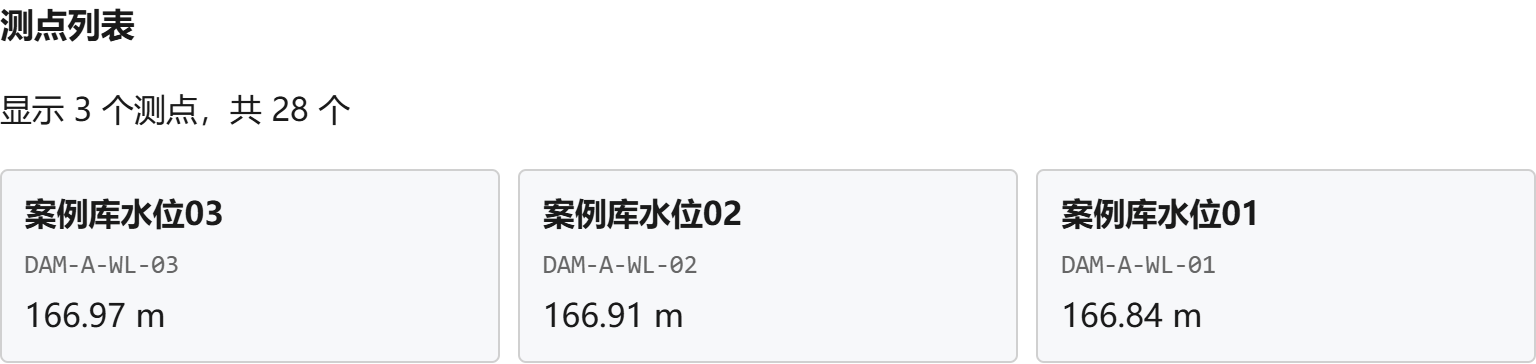
\includegraphics[width=16cm]{images/runtime/s1-asset-list.png}
\caption{S1测点列表的筛选与排序（配套阶段页实际运行截图）}
\label{fig:ch04-s1-list}
\end{figure}

\subsection{文档流、渲染流程与页面地标}

浏览器默认按标签在文件里的先后，从上到下、从左到右排列内容，这个默认顺序叫文档流。图\ref{fig:ch04-document-flow}展示同一份文档的两条处理路径：DOM与CSSOM合成后用于布局和绘制；DOM里的语义信息还用来生成可访问性树，读屏软件从中读出每个区域的角色、名称和状态。标签的先后顺序因此同时决定了阅读顺序和键盘操作顺序。监测页面先用文档流保证“标题—导航—数据—说明”的路径，再由CSS决定列数、间距和颜色。

\begin{figure}[htbp]
\centering
\begin{tikzpicture}[>=Stealth,thick,
  flow/.style={draw=Primary,rounded corners=2pt,text width=3.1cm,minimum height=.85cm,align=center,fill=PrimaryLight,text=PrimaryDark,font=\small}]
  \node[flow] (source) at (0,0) {HTML文档与CSS规则\\结构、语义和样式};
  \node[flow] (tree) at (4.4,0) {DOM / CSSOM\\浏览器内部对象};
  \node[flow] (render) at (8.8,0) {视觉渲染\\样式、布局、绘制合成};
  \node[flow] (access) at (4.4,-1.8) {可访问性树\\角色、名称和状态};
  \node[flow] (assist) at (8.8,-1.8) {辅助技术读取\\页面地标与内容};
  \draw[->,Primary] (source)--(tree);
  \draw[->,Primary] (tree)--(render);
  \draw[->,Primary] (tree)--node[left,font=\scriptsize]{依据DOM等信息}(access);
  \draw[->,Primary] (access)--(assist);
\end{tikzpicture}
\caption{语义化文档的视觉渲染与可访问性路径}
\label{fig:ch04-document-flow}
\end{figure}

一个元素脱离文档流（例如4.3.7节的绝对定位）后，后面的元素不会为它留出空间。整个监测面板都用绝对坐标拼接时，窗口尺寸或字体一变，内容就会互相遮挡，所以先用正常流表达层次，只在确实需要叠加的局部使用定位。页面出问题时，先判断它属于结构、样式还是脚本：开发者工具的“元素”面板检查DOM层级和可访问名称，“Computed”面板核对最终生效的样式，“性能”面板定位反复布局造成的卡顿，三者对应图\ref{fig:ch04-document-flow}的三个阶段。

渲染流程也决定了更新方式。水位数值每五分钟更新一次时，只替换输出节点的文本；趋势图一秒内收到多条消息时，先在内存中合并，再一次性刷新。

\paragraph{从地标到可访问名称}\texttt{header}放页面或区域的引导信息，\texttt{nav}放一组重要导航，\texttt{main}放页面唯一的主要内容，\texttt{section}是有主题标题的内容组，\texttt{article}是能独立发布的报告或公告，\texttt{aside}放辅助信息，\texttt{footer}放来源与更新时间，\texttt{figure}与\texttt{figcaption}把图表和说明绑在一起。这些区域统称页面地标，读屏用户可以按地标列表直接跳到“实时监测”或“预警事件”。选标签看内容的职责，不看浏览器给它的默认样式：有标题、能脱离周围内容单独理解的监测卡片用\texttt{article}；几个同类指标的分组用带标题的\texttt{section}；只为排版而设的容器用\texttt{div}。\texttt{main}在一个文档中只能有一个，标题从\texttt{h1}逐级向下，不为了字号跳级。

清单\ref{lst:ch04-a41-landmarks}把清单\ref{lst:ch04-html-shell}的\texttt{<body>}换成带地标的监测页面。开头的\texttt{href="\#monitor-main"}是“跳到主要内容”链接，键盘用户不必每次经过全局导航；\texttt{aria-labelledby}把区域标题与地标关联起来；\texttt{tabindex="-1"}只让脚本能把焦点移到主要内容，不会把它加入 Tab 键的遍历顺序。水位数字放在\texttt{output}里，并用\texttt{aria-live="polite"}声明“数值变化时请读屏软件在空闲时播报”；只有需要通知用户的数值才加这个属性，否则每个传感器的细小波动都会打断值班员。用浏览器打开后按 Tab 键，第一个获得焦点的应是跳转链接。

\begin{lstlisting}[label={lst:ch04-a41-landmarks},language=html,caption={带地标和跳转链接的监测页面（只列 body 部分）}]
<body>
  <a class="skip-link" href="#monitor-main">跳到主要内容</a>
  <header>
    <h1>水利工程安全监测平台</h1>
    <p>面向值班员的实时监测工作台</p>
  </header>
  <nav aria-label="主导航">
    <a href="#monitor-main">实时监测</a>
    <a href="#warning-panel">预警事件</a>
    <a href="#data-note">数据说明</a>
  </nav>
  <main id="monitor-main" tabindex="-1">
    <h2>实时监测</h2>
    <section aria-labelledby="level-title">
      <h3 id="level-title">水位概览</h3>
      <p>当前水位：<output id="level" aria-live="polite">--</output> m</p>
      <figure>
        <div id="level-chart" role="img"
             aria-label="最近一小时水位趋势图"></div>
        <figcaption>最近一小时水位趋势（示意）</figcaption>
      </figure>
    </section>
    <aside id="warning-panel" aria-labelledby="warning-title">
      <h3 id="warning-title">预警事件</h3>
      <p id="warning-message" role="status">暂无需要处理的事件</p>
    </aside>
  </main>
  <footer id="data-note">
    <p>数据来源：水利工程安全监测平台；更新时间：
      <time datetime="2026-08-07T08:00:00+08:00">08:00</time></p>
  </footer>
</body>
\end{lstlisting}

\subsection{表单与原生校验}

地标回答“我现在在哪里”，表单控件回答“我能提交什么”。浏览器在提交前会按控件上的约束属性自动检查输入，这叫原生校验：\texttt{required}不允许空值，\texttt{pattern}用正则表达式检查编码格式，\texttt{min}、\texttt{max}和\texttt{step}限定数值范围和步长。清单\ref{lst:ch04-a41-form}用测站编码、开始时间和采样间隔演示这些属性。把它放进页面后不写任何脚本，编码留空直接点“查询”，浏览器会在输入框旁弹出默认的提示气泡并阻止提交，这就是原生校验在起作用。表单里预留的\texttt{role="alert"}段落先是空的：4.4节有了JavaScript以后，可以给\texttt{<form>}加上\texttt{novalidate}关掉默认气泡，改由脚本把提示文字写进这个段落。提示要告诉用户怎么改，例如“格式如 DAM-A-PZ-07”，只写“输入错误”没有用。

\begin{lstlisting}[label={lst:ch04-a41-form},language=html,caption={监测查询表单的原生校验与可访问提示}]
<form id="query-form">
  <fieldset>
    <legend>查询条件</legend>
    <label for="station-code">测站编码</label>
    <input id="station-code" name="stationCode" required
           pattern="DAM-[A-Z]-[A-Z]{1,2}-[0-9]{2}" placeholder="DAM-A-PZ-07"
           aria-describedby="station-help">
    <small id="station-help">格式：工程-分区-类型-序号，如 DAM-A-PZ-07</small>

    <label for="start-time">开始时间</label>
    <input id="start-time" name="startTime" type="datetime-local"
           required aria-describedby="time-help">
    <label for="sample-step">采样间隔（分钟）</label>
    <input id="sample-step" name="step" type="number"
           min="5" max="60" step="5" value="5" required>
    <small id="time-help">时间范围还需由服务端校验</small>
  </fieldset>
  <p id="query-error" role="alert" aria-live="assertive"></p>
  <button type="submit">查询</button>
</form>
\end{lstlisting}

前端校验只是为了让用户尽早发现明显错误，不能代替后端校验：浏览器里的脚本可以被禁用或改写，别人也可以绕过页面直接发HTTP请求。采样间隔在页面上限定为5的倍数，并不意味着后端可以相信收到的一定是5的倍数；测站是否属于当前用户的权限范围、起止时间是否有序、时间跨度是否超限，都只能由服务器判断。第5章用 Jakarta Validation 的\texttt{@Valid}在服务端重新检查。两层校验的规则来自同一份数据字典：编码格式、时区和允许的采样间隔必须一致。后端返回400时，前端按错误体里的\texttt{field}把提示写回对应输入框旁的说明节点，并保留用户已经填好的其他条件。

校验做得对不对，可以按输入逐条检查：编码为空时提示“请输入测站编码”；格式错误时给出示例“DAM-A-PZ-07”；采样间隔超出范围时说明允许区间；三个错误同时存在时，表单顶部汇总数量，字段旁保留各自的原因。提交成功后，焦点移到结果标题或第一条结果上。

\subsection{指导实践：键盘路径与可访问性检查}

值班员可能整班只用键盘操作，页面需要一条可预测的键盘路径：跳转链接最先获得焦点，随后是主导航、查询表单、数据卡片和预警区域。这个顺序由DOM顺序决定，不要用正整数\texttt{tabindex}人为重排。页面内的普通状态更新用\texttt{role="status"}，需要立即处理的异常用\texttt{role="alert"}。弹出详情对话框时，焦点要移到对话框标题，关闭后回到触发按钮；这段焦点管理脚本要用到4.4节的JavaScript，收在附录C的\ref{app:ext-fe-focus-list}节。

检查时用四种方式各过一遍：只用键盘，看有没有走不出去的焦点陷阱；把浏览器字号放大到200\%，看有没有横向滚动；用读屏软件，看能否读出标题与单位；用自动化检查工具，确认每个表单控件都有名称。对动态预警，再确认普通状态更新不会抢走焦点。本章对键盘、对比度与状态编码的要求以WCAG 2.2为依据\cite{wcag22}。迁移到Vue以后，\texttt{header}、\texttt{nav}和\texttt{main}仍原样写在模板里，数据变化只更新\texttt{output}、表格行或图表容器，这些检查同样适用。

\section{CSS样式与响应式布局}

\paragraph{本节层次}核心：4.3.1、4.3.2、4.3.3、4.3.4、4.3.5；指导实践：4.3.6；拓展：4.3.7、4.3.8。

\paragraph{进入本节所需知识}先读4.2节，能在HTML里找到元素、属性与层次；准备好清单\ref{lst:ch04-html-shell}的页面，边改样式边刷新观察。

CSS决定页面长什么样。一条规则由选择器和声明块组成：选择器指出“对哪些元素”，声明块写“用什么样式”。清单\ref{lst:ch04-css-responsive}是监测卡片的样式，保存为\texttt{monitor.css}，清单\ref{lst:ch04-html-shell}的\texttt{<link>}已经引用了它。开头的\texttt{--normal}和\texttt{--warning}是CSS自定义属性，也叫CSS变量：在\texttt{:root}上定义一次，别处用\texttt{var(--warning)}取值，改颜色只改一处。工程中用类选择器（以点开头）组织组件样式，不依赖很深的标签层级。

\begin{lstlisting}[label={lst:ch04-css-responsive},language=CSS,caption={监测卡片响应式样式}]
:root { --normal: #1677ff; --warning: #d46b08; }
.monitor-grid {
  display: grid;
  grid-template-columns: repeat(3, minmax(12rem, 1fr));
  gap: 1rem;
}
.monitor-card {
  padding: 1rem;
  border: 1px solid #d9e2ec;
  border-radius: .5rem;
  background: #fff;
}
.monitor-card--warning { border-left: .35rem solid var(--warning); }
@media (max-width: 768px) {
  .monitor-grid { grid-template-columns: 1fr; }
}
\end{lstlisting}

\texttt{@media (max-width: 768px)}是媒体查询：视口宽度不超过768像素时，花括号里的规则才生效，三列卡片改为单列。清单\ref{lst:ch04-html-shell}的\texttt{<body>}里还没有卡片，要看到这个效果，先把清单\ref{lst:ch04-monitor-grid-html}放进\texttt{<main>}：三张卡片用\texttt{.monitor-grid}包住，其中一张带\texttt{.monitor-card--warning}。

\begin{lstlisting}[label={lst:ch04-monitor-grid-html},language=html,caption={供 monitor.css 作用的三张监测卡片（放在 main 内）}]
<div class="monitor-grid">
  <article class="monitor-card"><h3>DAM-A-WL-01</h3><p>库水位 164.2 m</p></article>
  <article class="monitor-card monitor-card--warning"><h3>DAM-A-PZ-07</h3><p>渗压 186.1 kPa</p></article>
  <article class="monitor-card"><h3>DAM-A-RF-01</h3><p>雨量 0.0 mm</p></article>
</div>
\end{lstlisting}

刷新后三张卡片并排；把浏览器窗口慢慢拉窄，或者在开发者工具里打开设备模拟器，可以看到列数在768像素处切换为单列，PZ-07 那张卡片左侧始终有一条橙色边。响应式设计不只是缩小字号，还要调整列数、触控目标大小和信息的先后。

\subsection{盒模型与尺寸计算}

浏览器把每个元素当作一个矩形盒子，从内到外依次是内容区、内边距（\texttt{padding}）、边框（\texttt{border}）和外边距（\texttt{margin}），这就是盒模型。\texttt{width}和\texttt{height}默认只描述内容区，因此一个写成\texttt{width: 320px; padding: 16px; border: 1px solid}的监测卡片，水平方向实际占用 $320+16\times2+1\times2=354$ 像素；三个这样的卡片放进1024像素宽的网格，还要扣掉间隙。尺寸算不清楚，卡片就会意外换行，图表会被挤出容器。

工程中通常在全局写\texttt{box-sizing: border-box}，让声明的宽高包含内边距和边框，设计稿上的320像素就是盒子的外部尺寸。图\ref{fig:ch04-css-box-model}从外到内标出四层区域；在开发者工具里选中元素时，四种高亮颜色分别对应这四层。

\begin{figure}[htbp]
\centering
\begin{tikzpicture}[font=\small]
  \draw[fill=PrimaryLight,draw=Primary] (0,0) rectangle (10,4.6);
  \node[PrimaryDark] at (5,.34) {margin 外边距};
  \draw[fill=white,draw=PrimaryDark] (.6,.7) rectangle (9.4,3.9);
  \node[PrimaryDark] at (5,1.025) {border 边框};
  \draw[fill=ChapterBg,draw=Accent] (1.2,1.35) rectangle (8.8,3.25);
  \node[PrimaryDark] at (5,1.675) {padding 内边距};
  \draw[fill=white,draw=Accent] (1.8,2) rectangle (8.2,2.6);
  \node[PrimaryDark] at (5,2.3) {content 内容区};
\end{tikzpicture}
\caption{CSS 盒模型的四层尺寸关系}
\label{fig:ch04-css-box-model}
\end{figure}

清单\ref{lst:ch04-css-box-sizing}用一条规则把测站卡片、数值输出和图表容器纳入同一种盒模型。通配符\texttt{*}连同\texttt{::before}、\texttt{::after}生成的装饰一起命中，它们也不会把布局撑大。

\begin{lstlisting}[label={lst:ch04-css-box-sizing},language=CSS,caption={监测卡片的 border-box 盒模型}]
*, *::before, *::after {
  box-sizing: border-box;
}

.station-card {
  width: min(100%, 20rem);
  padding: 1rem;
  border: 1px solid #d9e2ec;
  margin: 0;
  background: #fff;
}

.station-card__value {
  min-height: 2.5rem;
  overflow-wrap: anywhere;
}
\end{lstlisting}

\paragraph{选择器、优先级与层叠}几条规则同时命中一个元素、又给同一属性设了不同的值时，浏览器要决定谁生效，这个决定过程叫层叠。先比选择器的优先级，它可以写成三元组 $(a,b,c)$：$a$ 统计 ID 选择器，$b$ 统计类、属性和伪类，$c$ 统计元素和伪元素。先比 $a$，相同再比 $b$，最后比 $c$；三元组都相同时，后写的覆盖先写的。优先级不是数选择器的个数：一个 ID 高于任意多个类，一个类高于任意多个元素选择器。表\ref{tab:ch04-css-specificity}用监测页面的三个选择器做了计算。

\begin{table}[H]
\centering
\caption{CSS 选择器优先级三元组示例}
\label{tab:ch04-css-specificity}
\begin{tabular}{p{0.28\textwidth}p{0.16\textwidth}p{0.42\textwidth}}
\toprule
选择器 & $(a,b,c)$ & 计算与应用场景 \\
\midrule
\texttt{\#monitor-main} & (1,0,0) & 页面主要区域的唯一标识，适合页面级布局边界 \\
\texttt{.station-card.warning} & (0,2,0) & 同时命中组件和状态类，用于预警卡片的局部样式 \\
\texttt{section output} & (0,0,2) & 两个元素选择器，作为低优先级默认样式 \\
\bottomrule
\end{tabular}
\end{table}

颜色或间距没有生效时，先在开发者工具的“样式”面板找到被划掉的声明，再按表中的三元组判断是谁覆盖了它。直接追加\texttt{!important}能让这一条强行生效，但下一个维护者只能再写一条更强的去压它，原因却始终没有找到；只在覆盖改不了的第三方组件时才用，并在注释里写明原因。

层叠之外还有继承：颜色、字体等属性会从父元素传给子元素，盒模型尺寸、外边距和定位不会。清单\ref{lst:ch04-css-cascade}里，\texttt{color}从\texttt{.dashboard}继承到卡片文字，\texttt{border-color}由状态类\texttt{.is-warning}显式覆盖。组件只依赖变量名，不关心页面用的是哪一种蓝色；\texttt{var()}的第二个参数是变量缺失时的后备值。

\begin{lstlisting}[label={lst:ch04-css-cascade},language=CSS,caption={主题变量与状态层叠规则}]
:root {
  --water-primary: #1565c0;
  --water-warning: #d46b08;
  --panel-gap: 1rem;
}

.dashboard {
  color: #263238;
  background: #f5f9ff;
}

.dashboard .station-card {
  border: 1px solid var(--water-primary, #1565c0);
  margin-block-end: var(--panel-gap);
}

.station-card.is-warning {
  border-color: var(--water-warning, #d46b08);
}
\end{lstlisting}

\subsection{单位体系与可伸缩界面}

写长度之前先想清楚它相对于什么。\texttt{px}用于边框、图标描边这类要稳定像素精度的细节；\texttt{em}相对于当前元素的字号，按钮内边距用它，文字放大时按钮跟着变大；\texttt{rem}相对于根元素\texttt{html}的字号，适合全站统一的间距和字号刻度；\texttt{vw}、\texttt{vh}相对于视口宽度和高度，用于大屏容器的比例尺寸；百分比通常相对于父元素的对应属性，用于列宽和进度条。

清单\ref{lst:ch04-css-units}在同一个监测面板里用到这几种单位。\texttt{min()}取两个值中较小的一个，\texttt{min(100\%, 92vw)}保证面板不超出屏幕；\texttt{clamp(最小值, 首选值, 最大值)}让字号和间距随窗口宽度平滑变化，又不会小到看不清或大到失控。\texttt{vh}用于整屏高度时，手机浏览器的地址栏会伸缩，关键按钮不要只放在视口最底部。写完后把浏览器字号设置调大再看一遍，用固定像素锁死的文字不会跟着放大。

\begin{lstlisting}[label={lst:ch04-css-units},language=CSS,caption={监测面板的 CSS 单位策略}]
:root { font-size: 16px; }

.monitor-shell {
  width: min(100%, 92vw);
  min-height: min(80vh, 48rem);
  padding: clamp(1rem, 2vw, 2rem);
  gap: clamp(.75rem, 1.5vw, 1.5rem);
}

.monitor-shell h2 {
  font-size: clamp(1.25rem, 1rem + 1vw, 2rem);
}

.monitor-shell button {
  padding: .6em 1em;
  min-height: 2.75rem;
}
\end{lstlisting}

\subsection{Flexbox：一维的告警工具栏}

Flexbox 把一个容器里的子元素沿一条线排开，这条线叫主轴，与它垂直的方向叫交叉轴。在容器上写\texttt{display: flex}开启；\texttt{flex-direction}决定主轴方向，\texttt{justify-content}在主轴上分配剩余空间，\texttt{align-items}在交叉轴上对齐，\texttt{flex-wrap}允许放不下时换行，\texttt{gap}设置项目间距。子元素上的\texttt{flex}是三个值的缩写：有剩余空间时分多少（增长因子）、空间不够时缩多少（收缩因子）、分配前的基准尺寸。\texttt{flex: 1}表示可以分享剩余空间，不等于“固定等宽”，内容的最小宽度仍会参与计算。

告警工具栏是典型的一维布局：左侧放当前测站，中间放状态摘要，右侧放刷新、导出和确认按钮。清单\ref{lst:ch04-a43-flex-toolbar}给出样式和\texttt{<body>}内容，放进清单\ref{lst:ch04-html-shell}的骨架（样式写进\texttt{<head>}里的\texttt{<style>}）即可打开。宽度足够时三部分排成一行；把窗口拉窄到\texttt{44rem}以下，三部分各占一行，按钮仍保持\texttt{2.75rem}的可触控高度。不要用\texttt{white-space: nowrap}把所有控件锁在一行，否则放大字体或换到小屏就会出现横向滚动。

\begin{lstlisting}[label={lst:ch04-a43-flex-toolbar},language=html,caption={告警工具栏 Flex 实例（style 与 body 部分）}]
  <style>
    :root { --normal: #1677ff; --warning: #d46b08; }
    * { box-sizing: border-box; }
    body { margin: 0; font: 16px system-ui, sans-serif; }
    .alert-toolbar {
      display: flex;
      align-items: center;
      flex-wrap: wrap;
      gap: .75rem 1rem;
      padding: .75rem 1rem;
      border-block-end: 1px solid #d9e2ec;
    }
    .alert-toolbar__station { flex: 1 1 12rem; min-width: 10rem; }
    .alert-toolbar__summary { flex: 2 1 16rem; }
    .alert-toolbar__actions {
      display: flex; align-items: center; flex-wrap: wrap; gap: .5rem;
    }
    .alert-toolbar button {
      min-height: 2.75rem; padding: .55em 1em; border: 1px solid #b0bec5;
      border-radius: .35rem; background: #fff; color: #263238;
    }
    .alert-toolbar button.primary {
      border-color: var(--normal); background: var(--normal); color: #fff;
    }
    @media (max-width: 44rem) {
      .alert-toolbar { align-items: stretch; }
      .alert-toolbar__station, .alert-toolbar__summary,
      .alert-toolbar__actions { flex-basis: 100%; }
    }
  </style>
  <!-- 以上放进 <head>，以下放进 <body> -->
  <header class="alert-toolbar" aria-label="告警工具栏">
    <strong class="alert-toolbar__station">案例水库·测站筛选</strong>
    <span class="alert-toolbar__summary" role="status">当前有 2 条待确认事件</span>
    <span class="alert-toolbar__actions">
      <button type="button">刷新</button>
      <button type="button">导出</button>
      <button class="primary" type="button">确认事件</button>
    </span>
  </header>
\end{lstlisting}

读这份清单时分清两类属性：\texttt{display:flex}、\texttt{flex-wrap}、\texttt{align-items}、\texttt{gap}写在容器上；\texttt{flex}、\texttt{min-width}写在项目上。项目属性里还有一个\texttt{order}，它只改变画出来的顺序，不改变DOM顺序、Tab 键顺序和读屏顺序。告警操作的DOM顺序保持“查看—确认—导出”的业务逻辑，视觉对齐交给轴属性。

\subsection{Grid：二维的监测仪表盘}

Grid 同时管理行和列，适合把侧栏、地图、曲线、预警列表和底部状态栏拼成一个版面。\texttt{grid-template-columns}描述每一列的宽度，\texttt{grid-template-rows}描述每一行的高度，\texttt{grid-template-areas}用名字画出各区域的位置；\texttt{1fr}表示“分一份剩余空间”，\texttt{minmax(最小, 最大)}给出轨道尺寸的范围，\texttt{repeat(auto-fit, minmax(10rem, 1fr))}让卡片列数随可用宽度自动增减。

图\ref{fig:ch04-layout-choice}给出两种布局的分工：只沿一条轴分配空间的工具栏用 Flexbox；要同时控制行列的页面骨架用 Grid；Grid 区域内部的按钮组可以继续用 Flexbox。两者可以混用，但每一层元素只承担一种布局职责。

\begin{figure}[htbp]
\centering
\begin{tikzpicture}[>=Stealth,thick,node distance=0.7cm and 1.2cm]
  \tikzset{choice/.style={draw=Primary,rounded corners=2pt,minimum width=3.5cm,minimum height=1.0cm,align=center,fill=PrimaryLight,text=PrimaryDark,font=\small},
    detail/.style={draw=Accent,rounded corners=2pt,minimum width=3.5cm,minimum height=0.75cm,align=center,fill=white,text=PrimaryDark,font=\small}}
  \node[choice] (flex) {Flexbox\\一维主轴};
  \node[choice,right=of flex] (grid) {Grid\\二维行列};
  \node[detail,below=of flex] (toolbar) {工具栏、按钮组、状态摘要};
  \node[detail,below=of grid] (dashboard) {侧栏、地图、曲线、告警区};
  \draw[->,draw=Primary] (flex)--(toolbar);
  \draw[->,draw=Primary] (grid)--(dashboard);
  \draw[<->,draw=Accent] (flex.east)--node[above,font=\scriptsize]{按层组合}(grid.west);
\end{tikzpicture}
\caption{Flexbox 与 Grid 的布局职责边界}
\label{fig:ch04-layout-choice}
\end{figure}

清单\ref{lst:ch04-a43-grid-dashboard}同样只列样式和\texttt{<body>}。宽屏时显示侧栏、主图区和预警栏三列；窗口窄于\texttt{62rem}时，媒体查询把区域重排为单列，顺序变为标题、主数据、预警、测站、页脚。HTML顺序始终按阅读顺序书写，Grid 只改变视觉位置。\texttt{.dashboard > *}上的\texttt{min-width: 0}允许格子里的长内容收缩，去掉它再放一个很长的测站名，可以看到格子被撑破。

\begin{lstlisting}[label={lst:ch04-a43-grid-dashboard},language=html,caption={监测仪表盘 Grid 实例（style 与 body 部分）}]
  <style>
    * { box-sizing: border-box; }
    .dashboard {
      display: grid;
      grid-template-areas:
        "header header header"
        "side main alerts"
        "footer footer footer";
      grid-template-columns: minmax(12rem, 18rem) minmax(0, 1fr) minmax(14rem, 22rem);
      grid-template-rows: auto minmax(20rem, 1fr) auto;
      gap: 1rem;
      min-height: 100vh;
      padding: 1rem;
      background: #f5f9ff;
    }
    .dashboard > * { min-width: 0; padding: 1rem; background: #fff; }
    .dashboard__header { grid-area: header; }
    .dashboard__side { grid-area: side; }
    .dashboard__main { grid-area: main; }
    .dashboard__alerts { grid-area: alerts; }
    .dashboard__footer { grid-area: footer; }
    .metric-cards {
      display: grid;
      grid-template-columns: repeat(auto-fit, minmax(10rem, 1fr));
      gap: .75rem;
    }
    @media (max-width: 62rem) {
      .dashboard {
        grid-template-areas: "header" "main" "alerts" "side" "footer";
        grid-template-columns: 1fr;
      }
    }
  </style>
  <!-- 以上放进 <head>，以下放进 <body> -->
  <main class="dashboard">
    <header class="dashboard__header"><h1>水利工程安全监测</h1></header>
    <aside class="dashboard__side"><h2>测站</h2><p>站点列表</p></aside>
    <section class="dashboard__main" aria-labelledby="metrics-title">
      <h2 id="metrics-title">实时指标</h2>
      <div class="metric-cards">
        <article><h3>水位</h3><p>—</p></article>
        <article><h3>流量</h3><p>—</p></article>
      </div>
    </section>
    <aside class="dashboard__alerts"><h2>预警事件</h2><p>暂无</p></aside>
    <footer class="dashboard__footer">数据更新时间：—</footer>
  </main>
\end{lstlisting}

\subsection{响应式断点}

媒体查询切换样式的那个宽度叫断点。断点设在内容开始拥挤或操作不便的位置，由真实卡片、表格和按钮的最小宽度推出来，不照抄某个手机型号的像素值；一个断点只解决一个看得见的问题，例如导航换行、侧栏折叠，或图表从并排改为上下排列。写法有两种方向：移动优先先写单列、可滚动、大触控目标的基础样式，再用\texttt{min-width}逐级加列；桌面优先先写宽屏，再用\texttt{max-width}收拢。清单\ref{lst:ch04-css-responsive}是桌面优先，下面的清单\ref{lst:ch04-a43-breakpoints}是移动优先。

图\ref{fig:ch04-responsive-breakpoints}给出窄视口和三个宽视口的布局示例，宽度以 CSS 像素计：1920像素时安排侧栏、主图和预警栏三列，2560与3840像素的值班室大屏增加留白和可见信息；窄视口优先保留水位、预警和更新时间，折叠次要的筛选条件。断点之间用流式尺寸过渡。

\begin{figure}[htbp]
\centering
\begin{tikzpicture}[>=Stealth,thick]
  \draw[->,draw=Primary] (0,0)--(12,0);
  \foreach \x/\labeltext/\mode in {0/窄视口/单列,3.2/1920/三栏,7.0/2560/扩展留白,10.2/3840/多区布局} {
    \draw[draw=Primary] (\x,0.12)--(\x,-0.12);
    \node[align=center,font=\small,text=PrimaryDark] at (\x,0.52) {\labeltext};
    \node[align=center,font=\scriptsize,text=TextGray] at (\x,-0.48) {\mode};
  }
  \node[align=center,font=\small,text=PrimaryDark] at (6,1.15) {视口可用宽度（CSS px）\\按内容调整布局密度，刻度为非等距示意};
\end{tikzpicture}
\caption{监测平台的响应式断点与大屏适配思路}
\label{fig:ch04-responsive-breakpoints}
\end{figure}

清单\ref{lst:ch04-a43-breakpoints}里，基础样式是单列，三个\texttt{min-width}档位逐级设置三列的宽度；\texttt{aspect-ratio: 16 / 9}固定图表容器的宽高比，重排时高度不会跳动。根字号为16像素时，\texttt{120rem}就是1920像素。

\begin{lstlisting}[label={lst:ch04-a43-breakpoints},language=CSS,caption={移动优先与 1920/2560/3840 大屏断点}]
:root {
  --normal: #1677ff;
  --page-gap: clamp(.75rem, 1vw, 2rem);
  --content-max: 120rem;
}

.water-dashboard {
  width: min(100%, var(--content-max));
  margin-inline: auto;
  padding: var(--page-gap);
  display: grid;
  grid-template-columns: 1fr;
  gap: var(--page-gap);
}
.water-dashboard__chart { aspect-ratio: 16 / 9; min-height: 16rem; }
.water-dashboard__normal { color: var(--normal); }

@media (min-width: 120rem) { /* 1920 CSS 像素附近的宽屏 */
  .water-dashboard { grid-template-columns: 18rem minmax(0, 1fr) 22rem; }
}
@media (min-width: 160rem) { /* 2560 CSS 像素附近的宽屏 */
  .water-dashboard { --page-gap: 2rem; grid-template-columns: 22rem minmax(0, 1fr) 28rem; }
}
@media (min-width: 240rem) { /* 3840 CSS 像素附近的联屏 */
  .water-dashboard { --page-gap: 2.5rem; grid-template-columns: 26rem minmax(0, 1fr) 32rem; }
}
\end{lstlisting}

每个断点前后都检查同一件事：值班员能否完成同一项查询或确认任务，水位、预警等级和更新时间是否都还看得见，图表比例和按钮的可点击区域是否正常。

\subsection{指导实践：Flex布局的故障定位与可访问性验收}

页面出现“按钮被挤出屏幕”“摘要文字遮住数值”或“窄屏时卡片突然变高”时，先别急着加媒体查询，把问题还原成 Flex 的尺寸计算：容器的可用主轴空间等于自身宽度减去内边距、边框和间隙；每个项目先取\texttt{flex-basis}或自身内容的宽度作为基准，再按增长和收缩因子分配差额。项目有一个默认的最小宽度，等于它的内容不换行时的宽度；分配结果小于这个值时，浏览器保留最小宽度，于是出现横向溢出。对长测站名、单位文本和操作按钮，在项目上显式写\texttt{min-width: 0}解除这个下限，再在允许截断的地方配合\texttt{overflow-wrap}或省略号。

清单\ref{lst:ch04-a49-flex-debug}是一个便于诊断的告警摘要栏：外层容器分配主轴空间；中间的摘要\texttt{flex: 1 1 18rem}，宽屏时分享空间、窄屏时主动换行；右侧操作组\texttt{flex: 0 0 auto}，确认按钮不会被压成点不中的窄条。在开发者工具里逐条取消这些属性，可以看到横向溢出、换行和按钮大小分别由哪条规则决定。

\begin{lstlisting}[label={lst:ch04-a49-flex-debug},language=CSS,caption={可诊断的告警摘要 Flex 样式}]
.alert-summary {
  display: flex;
  align-items: center;
  flex-wrap: wrap;
  gap: .75rem 1rem;
  padding: .75rem 1rem;
  border: 1px solid #b0bec5;
}

.alert-summary__reading {
  flex: 1 1 18rem;
  min-width: 0;
  overflow-wrap: anywhere;
}

.alert-summary__reading strong {
  display: block;
  overflow: hidden;
  text-overflow: ellipsis;
  white-space: nowrap;
}

.alert-summary__actions {
  display: flex;
  flex: 0 0 auto;
  flex-wrap: wrap;
  gap: .5rem;
}

.alert-summary button {
  min-block-size: 2.75rem;
  padding-inline: 1rem;
}

@media (max-width: 36rem) {
  .alert-summary { align-items: stretch; }
  .alert-summary__reading,
  .alert-summary__actions { flex-basis: 100%; }
}
\end{lstlisting}

\paragraph{现象、原因与处理}表\ref{tab:ch04-flex-diagnostics}列出四种常见现象和对应的检查顺序。每次只改一个因素，然后在320、768、1280像素和联屏宽度下各看一遍，再只用键盘从页面标题走到筛选、查看、确认和导出，确认焦点环没有被\texttt{overflow:hidden}裁掉、视觉顺序与操作顺序一致；最后把浏览器字号放大到200\%，检查文字有没有被固定高度遮住。问题只出现在某一个测站名上时，修这个项目的最小宽度和断词方式，不要把整个页面改成固定宽度。

\begin{table}[htbp]
\centering
\caption{Flex布局常见现象与定位路径}
\label{tab:ch04-flex-diagnostics}
\begin{tabular}{p{0.24\textwidth}p{0.31\textwidth}p{0.31\textwidth}}
\toprule
现象 & 先检查 & 教学结论 \\
\midrule
右侧按钮被挤出 & 项目是否有\texttt{min-width:0}、按钮是否为\texttt{flex:0 0 auto} & 先保障操作命中区，再让摘要文本收缩 \\
窄屏出现横向滚动 & 容器的\texttt{flex-wrap}、长文本断词和固定宽度 & 换行是布局策略，不是异常补丁 \\
焦点顺序与视觉顺序不一致 & DOM 顺序、\texttt{order}和键盘 Tab 路径 & 语义顺序优先于视觉排列 \\
放大字号后文字被遮挡 & 固定高度、\texttt{overflow:hidden}和行高 & 组件高度应允许内容增长 \\
\bottomrule
\end{tabular}
\end{table}

预警状态不能只靠颜色表达。蓝、黄、橙、红之外还要有文字、图标或阈值说明；状态摘要用\texttt{role=status}，只有需要立即打断值班员的异常才用\texttt{role=alert}，轮询得到的每次普通更新都不应触发打断式播报。

\subsection{拓展：定位、层叠上下文与覆盖关系}

\texttt{position}有五种常用取值。\texttt{static}是默认值，元素留在文档流里；\texttt{relative}仍占着原位置，可以相对自身偏移，更常见的用途是给绝对定位的后代当参照；\texttt{absolute}脱离文档流，相对最近的已定位祖先摆放；\texttt{fixed}相对视口固定，适合始终可见的工具条，要留意它遮住内容；\texttt{sticky}在滚动到阈值后暂时固定，适合表头或测站分组标题。卡片网格这类整体布局仍然用 Grid 或 Flexbox，定位只处理局部的叠加。

几个元素叠在一起时，\texttt{z-index}大的在上面，但这个比较只在同一个层叠上下文里有效。层叠上下文可以理解为一个独立的图层组：组内元素先排好上下，再作为一个整体与组外元素比较。设置\texttt{transform}、小于1的\texttt{opacity}、\texttt{filter}等属性都会让元素自成一组，这时它的子元素写再大的\texttt{z-index}也盖不过组外的兄弟，“\texttt{z-index: 9999}不生效”多半是这个原因。监测地图上的预警浮层因此要划清图层边界：地图图层、测站详情、全局提示各占一组。

清单\ref{lst:ch04-css-position}里，工具条用\texttt{sticky}留在滚动容器顶部，浮层以相对定位的页面容器为参照；\texttt{isolation: isolate}显式创建一个层叠上下文，第三方地图内部的层级不会穿到业务提示上面。在页面里放一个长列表，滚动并切换浮层，观察定位和遮挡关系。

\begin{lstlisting}[label={lst:ch04-css-position},language=CSS,caption={监测工具条与预警浮层的定位}]
.monitor-page {
  position: relative;
  isolation: isolate;
}

.monitor-toolbar {
  position: sticky;
  top: 0;
  z-index: 10;
  display: flex;
  gap: .75rem;
  padding: .75rem 1rem;
  background: rgb(255 255 255 / .94);
}

.station-popover {
  position: absolute;
  inset: 3.5rem 1rem auto auto;
  z-index: 20;
  max-width: min(24rem, calc(100vw - 2rem));
  padding: 1rem;
  border: 1px solid #d46b08;
  background: #fffaf0;
}
\end{lstlisting}

\subsection{拓展：大屏缩放与暗色主题}

值班室大屏常见两种适配方案。\texttt{rem}方案以根字号为缩放基准，间距和字号成比例放大，文字保持清晰；\texttt{transform: scale()}方案把按固定像素排好的整张画布整体缩放，适合必须保持像素坐标的演示大屏，但字体、边框和可点击区域会一起缩放，还可能发虚或出现滚动条。日常使用的页面用\texttt{rem}加 Grid 做流式布局，只在只读的展示容器上使用整体缩放。

夜间值班需要暗色主题。做法是把文字、背景、边框和状态颜色都定义成CSS变量，在页面根元素上切换\texttt{data-theme}属性来替换整组变量值，组件样式不用改。暗色主题不是把白换成黑：文字与背景的对比度、曲线之间的区分度、预警色在暗底上的可见性和焦点环都要重新检查。主题由用户通过按钮或系统偏好选择，不随预警等级自动切换。完整的明暗主题与高对比度样式见附录C的\ref{app:ext-fe-theme}节。

\section{JavaScript基础编程}

\paragraph{本节层次}核心：4.4.1、4.4.2、4.4.3、4.4.4、4.4.5、4.4.7、4.4.8；指导实践：4.4.6。

\paragraph{进入本节所需知识}学过任意一门编程语言（Python、C、Java 均可），会写变量、分支、循环和函数；读过4.2节，知道页面是一棵由标签组成的树。

HTML和CSS写好的页面是静止的。点击按钮后筛选测点、输入编码后判断格式、向接口要数据再写进页面，都由JavaScript完成。本节的代码有两种运行方式：在浏览器里按 F12 打开“控制台”，把代码粘进去回车；或者保存为\texttt{.mjs}文件，用\texttt{node 文件名.mjs}执行。涉及\texttt{document}的代码操作的是页面，只能在浏览器里运行。

\paragraph{从已学语言到 JavaScript}变量、分支、循环和函数的用法与你学过的语言相差不大，\texttt{if}、\texttt{for}、\texttt{while}的写法与 C、Java 几乎相同。真正需要适应的差别不多，表\ref{tab:ch04-js-bridge}把它们列在一起，后面各小节逐项展开。

\begin{table}[htbp]
\centering
\caption{从 Python、C、Java 转到 JavaScript 时要留意的差别}
\label{tab:ch04-js-bridge}
\small
\begin{tabular}{p{2.1cm}p{5.3cm}p{6.2cm}}
\toprule
主题 & JavaScript 的写法 & 与已学语言的差别 \\
\midrule
变量 & \texttt{const limit = 165.5;}\newline \texttt{let count = 0;} & 声明时不写类型，类型跟着值走，同一个变量先后可以存字符串和数字；\texttt{const}声明后不能重新赋值，\texttt{let}可以 \\
相等 & \texttt{a === b}、\texttt{a !== b} & \texttt{==}会先转换类型再比较，\texttt{"5" == 5}为真；本书一律用三个等号，见4.4.1节 \\
空值 & \texttt{null}、\texttt{undefined} & 两种“空”：\texttt{null}是程序主动写入的“没有值”；读取对象上不存在的字段得到\texttt{undefined}，不会报错 \\
对象 & \texttt{\{ assetId: 'DAM-A-PZ-07',}\newline \texttt{\ \ value: 185.09 \}} & 不必先定义类，花括号直接写出一个对象，相当于 Python 的字典；用\texttt{reading.value}取字段。接口返回的 JSON 就是这种写法 \\
函数 & \texttt{function f(x) \{ return x * 2; \}}\newline \texttt{const f = x => x * 2;} & 函数本身是一个值，可以赋给变量、当作参数传给别的函数；第二行是箭头函数，是第一行的简写，见4.4.2节 \\
处理列表 & \texttt{list.filter(x => x > 1)}\newline \texttt{\ \ \ \ .map(x => x * 2)} & 相当于 Python 的列表推导式或 Java 的 stream；传进去的箭头函数对每个元素执行一次 \\
模块 & \texttt{import \{ f \} from './m.js';} & 路径相对于当前文件，扩展名要写全；被导入的文件用\texttt{export}标出对外公开的函数，见4.4.3节 \\
等待结果 & \texttt{const r = await fetch(url);} & 网络请求不会让程序停下来等；结果用 Promise 表示，\texttt{await}只暂停当前函数，见4.5.1节 \\
\bottomrule
\end{tabular}
\end{table}

基本类型有数字、字符串、布尔值、\texttt{null}、\texttt{undefined}，以及较少用到的\texttt{bigint}与\texttt{symbol}；数字不区分整数和浮点数。对象、数组和函数是引用类型，赋值和传参时传的是引用。字符串用单引号或双引号都可以；用反引号写的是模板字面量，里面的\texttt{\$\{表达式\}}会被替换成表达式的值，相当于 Python 的 f-string。

清单\ref{lst:ch04-js-basics}判断案例水库的实测水位是否越过汛限水位 165.5 m（取自表\ref{tab:case-parameters}）。粘进控制台运行，输出一行“案例库水位01：166.84 m，预警”；把\texttt{value}改成 165.12 再运行，输出变为“正常”。第四行的\texttt{条件 ? 甲 : 乙}是三元表达式，与 C、Java 相同。

\begin{lstlisting}[label={lst:ch04-js-basics},language=JavaScript,caption={JavaScript基础变量与函数}]
const stationName = "案例库水位01";
const warningLevel = 165.5; // 单位：m，案例水库汛限水位（8.1 节参数表）
const reading = { assetId: "DAM-A-WL-01", value: 166.84, unit: "m" };
const status = reading.value >= warningLevel ? "预警" : "正常";
const message = `${stationName}：${reading.value} ${reading.unit}，${status}`;
console.log(message.trim());
\end{lstlisting}

数组的\texttt{filter()}留下满足条件的元素，\texttt{map()}把每个元素换成另一个值，\texttt{reduce()}把整个数组合并成一个结果。清单\ref{lst:ch04-js-condition}先用前两个方法筛出越过汛限的观测并包装成对象，\texttt{alarms}的结果是只含 166.84 的一个元素。\texttt{validateLevel}把“不是数字”和“超出测点量程”当成两类错误分别抛出；如果两种情况都只返回\texttt{false}，调用方无从知道错在哪里。

\begin{lstlisting}[label={lst:ch04-js-condition},language=JavaScript,caption={监测值条件判断}]
const readings = [165.12, 166.84, 165.37];          // 案例库水位01 三次观测，单位 m
const floodLimit = 165.5;                            // 汛限水位，见 8.1 节参数表
const alarms = readings
  .filter(level => level >= floodLimit)
  .map(level => ({ level, severity: "warning" }));

function validateLevel(level) {
  if (!Number.isFinite(level)) throw new TypeError("水位必须是数字");
  // 量程取自测点台账（配套数据集 stations.csv）：148.0–171.6 m，即死水位到校核洪水位
  if (level < 148 || level > 171.6) throw new RangeError("水位超出测点量程");
  return level;
}
\end{lstlisting}

\subsection{类型、相等性与可预测数据}

JavaScript 的变量不固定类型，接口传来的数值又常常是字符串，例如\texttt{"166.84"}。如果不处理，\texttt{"166.84" + 1}得到的是字符串\texttt{"166.841"}，因为加号遇到字符串就做拼接。监测数据进入页面时要先解析和校验：把字符串数值转成有限数字，把缺失值统一成\texttt{null}，后面的代码才能放心计算和比较。

比较一律用严格相等\texttt{===}和严格不等\texttt{!==}，它们不转换类型：\texttt{5 === "5"}为假，\texttt{null === undefined}也为假。\texttt{==}会先按一套复杂规则转换类型，空字符串、0 和\texttt{false}互相“相等”；对水位、流量这类数值，“读数为 0”和“没有读数”含义完全不同，混在一起会出事故。业务上确实要把几种空值同等对待时，先写一个函数显式地把它们统一，再比较统一后的结果。

清单\ref{lst:ch04-a44-types}的\texttt{parseLevel}就是这样一个入口函数：先识别三种空值，再把字符串转成数字，最后用\texttt{Number.isFinite}排除\texttt{NaN}（“不是数字”，\texttt{Number('abc')}的结果）和无穷大。返回值里的\texttt{kind}字段说明这条读数是缺测、无效还是有效，调用方按它决定显示、统计还是拒收。在控制台里依次试\texttt{parseLevel('')}、\texttt{parseLevel('abc')}和\texttt{parseLevel('4.20')}，对照三种结果。

\begin{lstlisting}[label={lst:ch04-a44-types},language=JavaScript,caption={监测读数的类型守卫与严格比较}]
function parseLevel(raw) {
  if (raw === null || raw === undefined || raw === '') {
    return { kind: 'missing', value: null };
  }
  const value = typeof raw === 'number' ? raw : Number(raw);
  if (!Number.isFinite(value)) return { kind: 'invalid', value: null };
  return { kind: 'valid', value };
}

const reading = parseLevel('4.20');
if (reading.kind === 'valid' && reading.value === 4.2) {
  console.log('可以进入展示流程');
}
\end{lstlisting}

\subsection{函数、闭包与数组高阶方法}

函数在 JavaScript 里是一个值，可以存进变量、放进对象、传给别的函数，也可以作为返回值。\texttt{function}声明的命名函数适合表达稳定的业务操作；箭头函数\texttt{x => x * 2}适合写在\texttt{map}、\texttt{filter}的括号里。箭头右边只有一个表达式时，它的值就是返回值；要写多条语句就加花括号并显式\texttt{return}。

函数可以使用定义它的那一层作用域里的变量，而且在外层函数返回之后仍然能用，这种“函数连同它记住的变量”叫闭包。清单\ref{lst:ch04-a44-closures}的\texttt{makeRollingAverage}返回一个带\texttt{push}和\texttt{value}两个方法的对象，两个方法都记着同一个\texttt{samples}数组；外部代码拿不到\texttt{samples}，只能通过这两个方法操作它，效果相当于 Java 类的私有字段。要留意闭包记住的数据会一直占着内存：把很大的监测数组长期留在闭包里，页面切走后它也不会被回收，用完要主动放掉引用。

数组方法各有明确的用途：\texttt{map}改变每个元素的形状，\texttt{filter}筛选，\texttt{find}返回第一个满足条件的元素，\texttt{some}和\texttt{every}判断“存在”和“全部”，\texttt{reduce}把数组折叠成一个结果。清单后半段先用\texttt{filter}排除缺测的\texttt{null}，再用\texttt{reduce}求和，控制台输出两个有效值的平均数 166.2 附近的值（浮点运算的结果可能带很长的小数，显示时用\texttt{toFixed(2)}取两位）。每次链式调用都会产生一个新数组，对每秒多次到达的数据流，应先测量再决定要不要改成循环。

\begin{lstlisting}[label={lst:ch04-a44-closures},language=JavaScript,caption={闭包与数组高阶方法}]
function makeRollingAverage(limit = 3) {
  const samples = [];
  return {
    push(value) {
      if (Number.isFinite(value)) samples.push(value);
      if (samples.length > limit) samples.shift();
    },
    value() {
      return samples.length === 0
        ? null
        : samples.reduce((sum, item) => sum + item, 0) / samples.length;
    }
  };
}

const readings = [{ value: 166.1 }, { value: null }, { value: 166.3 }];
const validLevels = readings.map(item => item.value)
  .filter(level => Number.isFinite(level));
const average = validLevels.reduce((sum, level) => sum + level, 0)
  / validLevels.length;
console.log(average);
\end{lstlisting}

\subsection{解构、展开与 ES 模块}

解构是从对象或数组里一次取出多个字段的简写：\texttt{const \{ assetId, value \} = reading}等价于分别写\texttt{reading.assetId}和\texttt{reading.value}。解构时可以改名（\texttt{value: rawValue}），也可以给缺失字段指定默认值（\texttt{quality = 'missing'}）。展开语法\texttt{...}把一个对象的字段铺开到新对象里，\texttt{\{ ...summary, updated: true \}}得到一个多了\texttt{updated}字段的新对象，原对象不变。它只复制一层，嵌套的对象仍然是共用的。更新测站状态时总是创建新的顶层对象，避免一个组件改了对象，另一个组件的显示跟着变。

代码多了要分文件。JavaScript 标准的分文件方式叫 ES 模块：一个文件就是一个模块，用\texttt{export}标出对外公开的函数或常量，别的文件用\texttt{import}按名字导入，没有导出的内容外部看不见。模块按职责划分：\texttt{readings.js}负责解析和计算，\texttt{api.js}负责请求，页面代码只组合它们，状态不通过全局变量共享。在HTML里用\texttt{<script type="module" src="...">}引入入口模块，4.5节的阶段页就是这样组织的。\texttt{import}语句写在文件顶部，构建工具据此分析依赖；写成函数调用的\texttt{import('./map.js')}是动态导入，返回 Promise，可以把首屏用不到的地图或报表代码推迟到需要时再下载。

清单\ref{lst:ch04-a44-modules}在一个清单里列出两个文件。把它们放进 Vite 项目的\texttt{src/lib/}目录，在入口脚本里导入\texttt{station-panel.js}，控制台输出\texttt{\{ assetId: 'DAM-A-WL-01', value: 166.84, quality: 'valid', updated: true \}}；字符串\texttt{'166.84'}已经转成了数字，\texttt{response}本身没有被改动。

\begin{lstlisting}[label={lst:ch04-a44-modules},language=JavaScript,caption={ES 模块、解构与展开}]
// readings.js
export function summarizeReading(reading) {
  const { assetId, value: rawValue, quality = 'missing' } = reading;
  const value = rawValue === null ? null : Number(rawValue);
  return { assetId, value, quality };
}

// station-panel.js
import { summarizeReading } from './readings.js';

const response = { assetId: 'DAM-A-WL-01', value: '166.84', quality: 'valid' };
const summary = summarizeReading(response);
const viewModel = { ...summary, updated: true };
console.log(viewModel);
\end{lstlisting}

\subsection{DOM 查询、增删改与安全写入}

4.1节说过，浏览器把HTML解析成 DOM 树；JavaScript 通过全局对象\texttt{document}访问这棵树。\texttt{querySelector}按CSS选择器找到第一个匹配的节点，\texttt{querySelectorAll}找到全部；\texttt{closest}从一个节点向上找最近的匹配祖先，后面处理点击事件时要用。新增节点用\texttt{createElement}和\texttt{append}，删除用\texttt{remove}。HTML里以\texttt{data-}开头的自定义属性在脚本里通过\texttt{dataset}读写，\texttt{data-asset-id}对应\texttt{dataset.assetId}。

把外部数据写进页面时用\texttt{textContent}，它把内容当纯文本处理。\texttt{innerHTML}会把字符串当HTML解析，测站名称或事件说明里如果混进一段\texttt{<script>}或带事件属性的标签，就会在值班员的浏览器里执行，这类攻击叫 XSS（跨站脚本）。只有内容完全由自己的代码写死时才用\texttt{innerHTML}，清单开头搭页面结构的那一行属于这种情况。

清单\ref{lst:ch04-a44-dom}先在内存里的文档片段（\texttt{DocumentFragment}）上建好所有列表项，再用\texttt{replaceChildren}一次放进页面，浏览器只重新布局一次；逐个\texttt{append}到页面上则每次都可能触发布局。在任意页面的控制台里运行它，页面内容被替换成两行测点，第二行随后变成“案例渗压07：更新中”。

\begin{lstlisting}[label={lst:ch04-a44-dom},language=JavaScript,caption={安全创建和更新测站 DOM}]
document.body.innerHTML = '<ul id="station-list"></ul>';
const list = document.querySelector('#station-list');
const assets = [
  { assetId: 'DAM-A-WL-01', displayName: '案例库水位01', value: 166.84, unit: 'm' },
  { assetId: 'DAM-A-PZ-07', displayName: '案例渗压07', value: 185.09, unit: 'kPa' }
];

const fragment = document.createDocumentFragment();
for (const asset of assets) {
  const item = document.createElement('li');
  item.dataset.assetId = asset.assetId;
  item.textContent = `${asset.displayName}：${asset.value} ${asset.unit}`;
  fragment.append(item);
}
list.replaceChildren(fragment);
list.querySelector('[data-asset-id="DAM-A-PZ-07"]').textContent = '案例渗压07：更新中';
\end{lstlisting}

\subsection{事件对象、捕获与冒泡}

用户点击、输入、按键时，浏览器产生一个事件；用\texttt{addEventListener('click', 函数)}在某个节点上登记一个监听函数，事件发生时浏览器调用它，并传入一个描述这次事件的事件对象。

点击列表里的一个按钮，收到通知的不只是按钮。事件沿 DOM 树走三段：先从\texttt{window}向下经过各层祖先到达目标，叫捕获阶段；在目标节点上触发，叫目标阶段；再从目标逐层向上回到\texttt{window}，叫冒泡阶段。监听函数默认在冒泡阶段被调用，所以在\texttt{<ul>}上登记的监听函数能收到它里面任何一个按钮的点击，图\ref{fig:ch04-a44-event-flow}画出了这条路径。事件对象的\texttt{target}是最初被点击的节点，\texttt{currentTarget}是当前正在执行监听函数的节点；在\texttt{<ul>}上监听时，前者是按钮，后者是\texttt{<ul>}。4.4.6节的事件委托就建立在这个区别上。

\begin{figure}[htbp]
\centering
\begin{tikzpicture}[>=Stealth,thick,node distance=.7cm,
  event/.style={draw=Primary,rounded corners=2pt,text width=6.0cm,minimum height=.85cm,align=center,fill=PrimaryLight,text=PrimaryDark,font=\small}]
  \node[event] (capture) {捕获阶段\\window → document → list};
  \node[event,below=of capture] (target) {目标阶段\\被点击的元素（target）};
  \node[event,below=of target] (bubble) {冒泡阶段\\list → document → window};
  \draw[->,Primary] (capture)--(target);
  \draw[->,Primary] (target)--(bubble);
  \node[align=left,font=\scriptsize,text=TextGray,right=.65cm of target]
    {target：原始目标\\currentTarget：当前监听节点\\图中省略其他祖先元素};
\end{tikzpicture}
\caption{列表项 click 事件的捕获、目标与冒泡阶段}
\label{fig:ch04-a44-event-flow}
\end{figure}

事件对象还有两个常用方法。\texttt{preventDefault()}取消浏览器的默认动作，例如阻止表单提交后整页刷新、阻止链接跳转。\texttt{stopPropagation()}让事件不再继续传播，祖先节点上的监听函数就收不到它了；它会让上层组件“看不见”这次操作，除非确有必要，不用它来解决重复触发的问题。需要在捕获阶段监听时，把\texttt{addEventListener}的第三个参数写成\texttt{\{ capture: true \}}。

\subsection{事件委托与长列表}

28个测点的列表，如果给每个按钮各登记一个监听函数，列表每次重画都要重新登记。事件委托只在稳定的父容器上登记一个监听函数，靠冒泡接收所有子项的点击，再用\texttt{event.target.closest()}判断点中的是哪一项。列表新增项目不用再登记，监听函数的数量也不随测点数增长。

清单\ref{lst:ch04-a44-events}包含两段：第一段是\texttt{<ul>}上的事件委托，\texttt{closest('button[data-asset-id]')}找到被点击的按钮，\texttt{contains}确认它确实在本列表内，点击列表空白处时\texttt{button}为\texttt{null}，函数直接返回；第二段用\texttt{preventDefault}阻止链接跳转，改为在当前页面更新文字。在控制台运行后点击两个按钮，\texttt{output}里依次显示所选对象编码。按钮元素的\texttt{click}事件同时响应鼠标和键盘回车，不要改成只监听\texttt{mousedown}。

\begin{lstlisting}[label={lst:ch04-a44-events},language=JavaScript,caption={测站列表的事件委托与 preventDefault}]
document.body.innerHTML = `
  <a id="station-link" href="/assets">测站列表</a>
  <ul id="delegated-list">
    <li><button data-asset-id="DAM-A-WL-01">案例库水位01</button></li>
    <li><button data-asset-id="DAM-A-PZ-07">案例渗压07</button></li>
  </ul>
  <output id="delegated-result" aria-live="polite"></output>`;

const delegatedList = document.querySelector('#delegated-list');
const output = document.querySelector('#delegated-result');
delegatedList.addEventListener('click', event => {
  const button = event.target.closest('button[data-asset-id]');
  if (!button || !delegatedList.contains(button)) return;
  output.textContent = `选择了 ${button.dataset.assetId}`;
});

document.querySelector('#station-link').addEventListener('click', event => {
  event.preventDefault();
  output.textContent = '已在当前页面打开测站列表';
});
\end{lstlisting}

请求还没返回时，按钮要显示忙碌状态，不要再登记一个监听函数。列表很长时，瓶颈在节点数量和布局计算：几百行以内用分页或分组折叠；上万行才需要只渲染可视区域的虚拟滚动，它要处理行高估计、占位空间和键盘焦点，实现思路见附录C的\ref{app:ext-fe-focus-list}节。

\subsection{异常处理}

\texttt{try}包住可能失败的操作，\texttt{catch}处理异常，\texttt{finally}无论成败都执行，用来做清理，三者的用法与 Java、Python 的异常处理相同。\texttt{throw}可以抛出任何值，习惯上抛\texttt{Error}或它的子类，\texttt{instanceof}用来判断异常属于哪一类。异常不能悄悄吞掉：界面上给出值班员看得懂的提示，技术细节写进日志。清单\ref{lst:ch04-js-array}按异常类型分流，它调用了清单\ref{lst:ch04-js-condition}的\texttt{validateLevel}：报文不是合法 JSON、数值超出量程、其他未知失败各对应一个固定的错误码，界面按错误码决定提示文案。分别传入\texttt{'\{bad'}、\texttt{'\{"value":999\}'}和\texttt{'\{"value":166.84\}'}，对照三种返回值。

\begin{lstlisting}[label={lst:ch04-js-array},language=JavaScript,caption={监测报文解析的分类异常处理}]
function parseReading(raw) {
  try {
    const reading = JSON.parse(raw);
    return { ok: true, value: validateLevel(reading.value) };
  } catch (error) {
    if (error instanceof SyntaxError) {
      console.error("监测报文格式错误", error);
      return { ok: false, code: "MALFORMED_JSON", message: "数据格式无法解析" };
    }
    if (error instanceof RangeError) {
      console.warn("监测值超出量程", error);
      return { ok: false, code: "OUT_OF_RANGE", message: "数值超出测站量程" };
    }
    console.error("监测数据处理失败", error);
    return { ok: false, code: "UNKNOWN", message: "数据暂不可用" };
  }
}
\end{lstlisting}

\subsection{综合练习：测点编码输入与校验}

这个练习把 DOM 查询、事件监听和安全写入连起来：HTML 定义输入框、按钮和输出区，JavaScript 在点击时读取输入、判断、写回结果。阈值取案例水库的汛限水位 165.5 m（8.1节参数表）。清单\ref{lst:ch04-html-vue}放进清单\ref{lst:ch04-html-shell}骨架的\texttt{<main>}里。

\begin{lstlisting}[label={lst:ch04-html-vue},language=html,caption={测站输入 HTML 片段}]
<label for="level-input">库水位（m）</label>
<input id="level-input" type="number" step="0.01">
<button id="check-level" type="button">判断状态</button>
<output id="level-result" aria-live="polite"></output>
\end{lstlisting}

清单\ref{lst:ch04-a44-dom-script}保存为\texttt{check.js}，在\texttt{</body>}之前用\texttt{<script type="module"}\allowbreak\texttt{ src="check.js">}\allowbreak\texttt{</script>}引入。输入 166.84 点击按钮，输出区显示“超过汛限水位”；输入 165 显示“水位正常”；什么都不填直接点击，\texttt{Number('')}得到 0，页面显示“水位正常”，这是一个需要你修的缺陷：参照清单\ref{lst:ch04-a44-types}的\texttt{parseLevel}，让空输入得到“请输入有效水位”。

\begin{lstlisting}[label={lst:ch04-a44-dom-script},language=JavaScript,caption={测站输入 JavaScript 片段}]
const input = document.querySelector('#level-input');
const result = document.querySelector('#level-result');
const button = document.querySelector('#check-level');

button.addEventListener('click', () => {
  const level = Number(input.value);
  if (!Number.isFinite(level)) {
    result.textContent = '请输入有效水位';
    return;
  }
  result.textContent = level >= 165.5 ? '超过汛限水位' : '水位正常';
});
\end{lstlisting}

\section{数据请求与页面状态}\label{sec:ch04-request-state}

\paragraph{本节层次}核心：4.5.1、4.5.2、4.5.3、4.5.4、4.5.10；指导实践：4.5.5、4.5.6、4.5.7；拓展：4.5.8、4.5.9。

\paragraph{进入本节所需知识}4.4节的函数、数组方法、模块与 DOM 写入；会打开开发者工具的“网络”面板查看一次请求的状态码与耗时（见附录B的 P0 单元）；看过表\ref{tab:api-contract}中“对象列表”与“最新观测”两个端点的字段。本节不用自己写后端：配套工程的教学接口\texttt{teaching-api}按同一份契约、用固定数据集应答；第5章的后端完成认证与数据存储后，可以直接替换教学接口，页面代码不用改。

\paragraph{业务问题}值班员打开测点详情页，要看到该测点的最新观测值、时间和质量码。页面必须先显示“正在读取”，再显示数据或“暂无观测”，请求失败时说明原因；值班员连续点击两个测点时，最后显示的必须是最后点击的那个。本节最后交付的是一个能在教学接口上运行、四种状态都能观察到的详情页脚本，它也是 4.6 节 Vue 组件和 4.7 节 Pinia 仓库的前身。

\subsection{原理：一次请求从发出到页面更新}

在 Python 或 Java 里读文件、查数据库，程序通常停在那一行等结果。浏览器不能这样等：JavaScript 和页面绘制共用一个线程，等待网络的几百毫秒里如果停住，页面就无法滚动和点击。所以\texttt{fetch}发出请求后立刻返回，返回的不是数据，而是一个代表“将来才有的结果”的对象，叫 Promise。Promise 有三种状态：刚创建时是 pending（等待中），成功后变为 fulfilled（已兑现），失败后变为 rejected（已拒绝）。状态一旦落定就不再改变。用\texttt{then}登记成功后要做的事，用\texttt{catch}登记失败后要做的事；\texttt{then}本身又返回一个新的 Promise，因此可以一环接一环地写“取响应→解析 JSON→校验字段”。

清单\ref{lst:ch04-a45-promise}手工创建一个 Promise，并故意多次调用\texttt{resolve}和\texttt{reject}：只有第一次调用有效，后面的调用不会覆盖已经落定的结果。每个请求的 Promise 都遵守这条规则；两个不同请求谁先谁后则没有保证，要按 4.5.4 节的办法单独控制。

\begin{lstlisting}[label={lst:ch04-a45-promise},language=JavaScript,caption={Promise 状态一经落定不可再变}]
let resolveReading;
let rejectReading;
const readingPromise = new Promise((resolve, reject) => {
  resolveReading = resolve;
  rejectReading = reject;
});

readingPromise
  .then(value => console.log('fulfilled:', value))
  .catch(error => console.error('rejected:', error));

resolveReading({ value: 185.091, unit: 'kPa' });
rejectReading(new Error('这次调用不会改变状态'));
resolveReading({ value: 185.2, unit: 'kPa' });
// 控制台只输出一行：fulfilled: { value: 185.091, unit: 'kPa' }
\end{lstlisting}

\texttt{then}链写长了不好读。在函数前加\texttt{async}，函数内部就可以用\texttt{await}等一个 Promise 落定：成功时\texttt{await}表达式的值就是结果，失败时在这一行抛出异常，用普通的\texttt{try/catch}接住。\texttt{await}只暂停它所在的这个 async 函数，浏览器照常响应用户操作；async 函数的返回值总是一个 Promise。几个互不依赖的请求用\texttt{Promise.all}同时发出，全部成功才算成功，任何一个失败整体就失败；希望部分结果仍然可用时改用\texttt{Promise.allSettled}逐项检查。清单\ref{lst:ch04-js-fetch}与清单\ref{lst:ch04-js-debug}分别用\texttt{then}链和\texttt{async/await}读取同一个端点，路径来自表\ref{tab:api-contract}。要注意\texttt{fetch}只在网络不通时才失败，服务器返回 404 或 500 时它仍然“成功”，所以两份清单都先检查\texttt{response.ok}；204 表示没有响应体，不能再调用\texttt{json()}。

\begin{lstlisting}[label={lst:ch04-js-fetch},language=JavaScript,caption={then 链写法：读取一个对象的最新观测}]
function loadLatest(assetId) {
  return fetch(`/api/assets/${assetId}/readings/latest`)
    .then(response => {
      if (!response.ok) throw new Error(`HTTP ${response.status}`);
      return response.status === 204 ? null : response.json();
    });
}

loadLatest('DAM-A-PZ-07')
  .then(reading => console.log('最新观测', reading?.value, reading?.unit))
  .catch(error => console.error('加载失败', error));
\end{lstlisting}

\begin{lstlisting}[label={lst:ch04-js-debug},language=JavaScript,caption={async/await 写法：并发读取最新观测与该对象的预警}]
async function loadDetail(assetId) {
  try {
    const [latest, warnings] = await Promise.all([
      fetch(`/api/assets/${assetId}/readings/latest`),
      fetch(`/api/warnings?assetId=${assetId}`)
    ]);
    if (!latest.ok || !warnings.ok) throw new Error('接口响应异常');
    return { latest: latest.status === 204 ? null : await latest.json(),
             warnings: await warnings.json() };
  } catch (error) {
    console.error('详情加载失败', error);
    throw error;
  }
}
\end{lstlisting}

这两份清单的请求都没有带\texttt{Authorization}头，而表\ref{tab:api-contract}里除登录以外的接口都要求令牌，所以直接在控制台运行它们会得到“HTTP 401”并走进\texttt{catch}分支。登录前出现 401 是预期结果，4.5.2节讲完令牌怎样取得和附在请求上以后，这两个函数才能拿到数据。失败按来源分类处理：JSON 解析失败是输入格式错误，量程校验失败是业务数据错误，401 表示登录状态失效，5xx 表示服务端暂时不可用，超时或断网属于连接问题。契约把错误体统一为\texttt{\{code, message, field\}}，页面按状态码和\texttt{code}分流，不解析\texttt{message}里的自然语言文案。

\subsection{完整例子：读取对象列表与最新观测}

清单\ref{lst:ch04-r1-load}是本节的起点包：登录取得令牌，读取对象列表，找到渗压计 \texttt{DAM-A-PZ-07}，把它的最新观测写进页面。它只用浏览器自带的\texttt{fetch}，没有任何框架；\texttt{getJson}集中处理了契约规定的 204（尚无观测）与错误体，页面层不必各自解析响应。

\begin{lstlisting}[label={lst:ch04-r1-load},language=JavaScript,caption={detail.js：登录、对象列表与最新观测（S2 阶段起点）}]
// 开发时由 Vite 代理把 /api 转发到教学接口或真实后端（见 4.5.6）
let token = null;

export async function login(username, password) {
  const res = await fetch('/api/auth/login', {
    method: 'POST',
    headers: { 'Content-Type': 'application/json', Accept: 'application/json' },
    body: JSON.stringify({ username, password })
  });
  if (!res.ok) throw new Error(`LOGIN_${res.status}`);
  token = (await res.json()).accessToken;
}

async function getJson(path, signal) {
  const res = await fetch(path, {
    headers: { Accept: 'application/json', Authorization: `Bearer ${token}` },
    signal
  });
  if (res.status === 204) return null;                // 契约：尚无观测
  if (!res.ok) {
    const body = await res.json().catch(() => ({}));  // 契约：{code, message, field?}
    throw Object.assign(new Error(body.code ?? `HTTP_${res.status}`),
                        { status: res.status, body });
  }
  return res.json();
}

export const loadAssets = () => getJson('/api/assets');
export const loadLatest = (assetId, signal) =>
  getJson(`/api/assets/${encodeURIComponent(assetId)}/readings/latest`, signal);

export function renderLatest(el, asset, reading) {
  if (!reading) { el.textContent = `${asset.displayName}：暂无观测`; return; }
  el.textContent = `${asset.displayName}：${reading.value} ${reading.unit}`
    + `（${reading.occurredAt}，质量 ${reading.quality}）`;
}

// 页面入口（index.html 中 <p id="latest"></p> 与 <script type="module" src="/src/detail.js">）
const output = document.querySelector('#latest');
await login('duty01', 'duty123');
const assets = await loadAssets();
const pz07 = assets.find(a => a.assetId === 'DAM-A-PZ-07');
renderLatest(output, pz07, await loadLatest(pz07.assetId));
\end{lstlisting}

\paragraph{页面入口与可导入模块}清单末尾的页面入口（查\texttt{\#latest}、登录、渲染 PZ-07）能直接写在模块顶层，是因为此刻\texttt{detail.js}是页面唯一的脚本；\texttt{await}写在模块顶层也是 ES 模块允许的。4.5.4 节加入入口文件\texttt{main.js}之后要把这几行删掉：模块顶层的语句在被\texttt{import}的那一刻就会执行，留着它，每次导入都会重新登录一次，并抢在列表渲染之前先画一次 PZ-07；写单元测试时导入\texttt{controller.js}也会被它带着发真实请求。删掉之后登录改由\texttt{main.js}负责，\texttt{detail.js}成为一个只导出函数的模块，配套工程\texttt{frontend/src/lesson45/}里的就是删掉之后的版本。

\paragraph{运行方式}在配套工程目录执行\texttt{node teaching-api/server.mjs}启动教学接口（默认 8080 端口），再在\texttt{frontend}目录执行\texttt{npm run dev}启动 Vite 开发服务器，浏览器打开它给出的地址。Vite 的代理把\texttt{/api}转发到 8080，因此脚本里只写相对路径。

\paragraph{可观察结果}页面出现一行文字：“案例渗压07：185.091 kPa（2026-07-01T23:55:00+08:00，质量 valid）”。开发者工具“网络”面板依次出现三条请求：\texttt{POST /api/auth/login} 返回 200，\texttt{GET /api/assets} 返回 200 且响应体是 28 个对象的数组，\texttt{GET /api/assets/DAM-A-PZ-07/readings/latest} 返回 200。把最后一条的地址复制到新标签页直接打开，得到的是 401：地址栏访问不带\texttt{Authorization}头，受保护接口按契约拒绝没有令牌的请求。表\ref{tab:ch04-r1-run}把这几条请求与页面结果对应起来。

\begin{table}[htbp]
\centering
\caption{清单\ref{lst:ch04-r1-load}的预期运行记录（教学接口 + 固定数据集）}
\label{tab:ch04-r1-run}
\begin{tabular}{p{0.36\textwidth}p{0.12\textwidth}p{0.42\textwidth}}
\toprule
请求 & 状态码 & 响应要点 / 页面变化 \\
\midrule
POST /api/auth/login & 200 & 响应含 accessToken，authorities 为 DUTY；页面无变化 \\
GET /api/assets & 200 & 数组长度 28（表\ref{tab:case-parameters}的测点总数）；页面无变化 \\
GET /api/assets/DAM-A-PZ-07/readings/latest & 200 & value 185.091、unit kPa、quality valid；页面写入一行文字 \\
同一地址在新标签页打开 & 401 & 错误体 code 为 UNAUTHORIZED；说明令牌只存在于脚本变量中 \\
\bottomrule
\end{tabular}
\end{table}

图\ref{fig:ch04-http-observe}是在“网络”面板里读一条请求的方法：先定位请求，再读状态码和响应字段。图中的请求把时间范围写反了，返回 400，错误体的\texttt{field}指向\texttt{from}。

\begin{figure}[htbp]
\centering
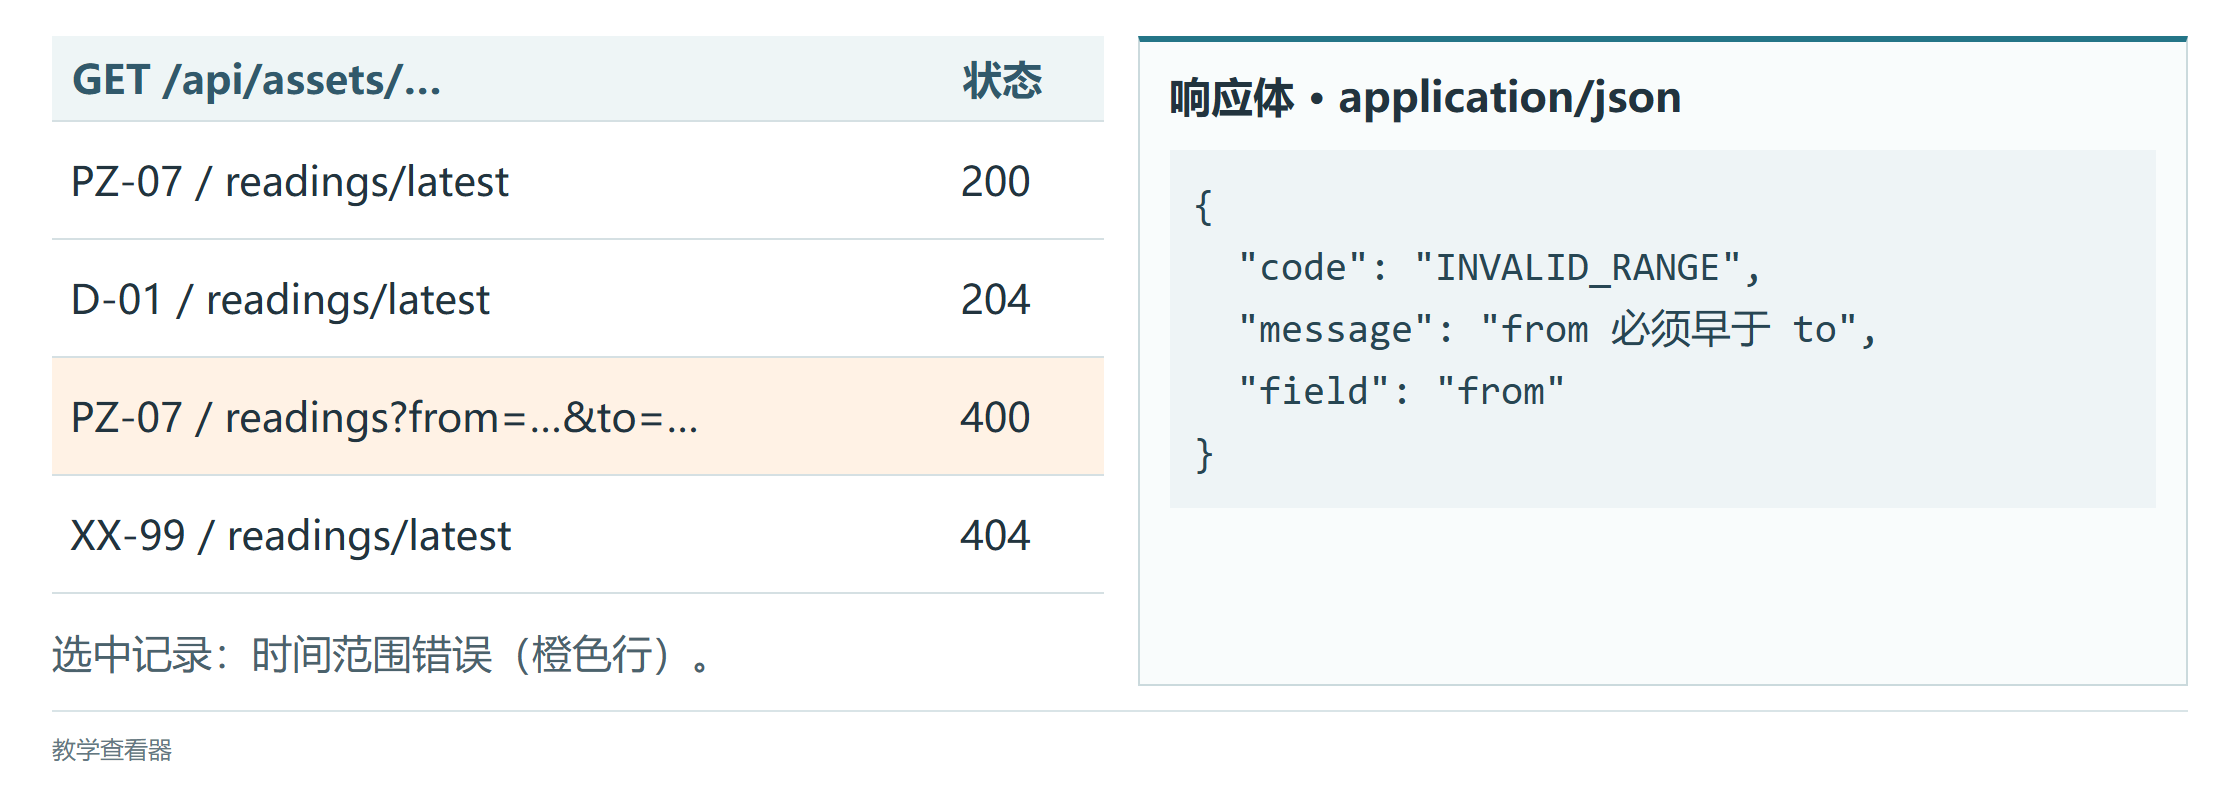
\includegraphics[width=16cm]{images/runtime/http-network-json.png}
\caption{请求状态与JSON响应对照（教学查看器，调用配套教学接口）}
\label{fig:ch04-http-observe}
\end{figure}

\subsection{页面的四种状态：加载、空数据、错误与过期}

清单\ref{lst:ch04-r1-load}只处理了“成功”这一条路。真实页面在任一时刻只能处于一种状态：正在加载、有数据、没有数据、出了错。把状态显式写成一个对象，渲染函数只看状态不看网络，后面的 Vue 组件与 Pinia 仓库也是这个做法。表\ref{tab:ch04-r1-states}列出四种状态、用教学接口触发它的方式（参数含义见表\ref{tab:api-teach-faults}）和页面应有的表现。还有一种情况是“过期”：请求发出后用户已经切到别的对象，这个请求即使返回结果也要丢弃，页面保持当前状态，处理方法见 4.5.4 节。

\begin{table}[htbp]
\centering
\caption{详情页的状态模型与教学接口触发方式}
\label{tab:ch04-r1-states}
\begin{tabular}{p{0.12\textwidth}p{0.30\textwidth}p{0.48\textwidth}}
\toprule
状态 & 触发方式 & 页面应有表现 \\
\midrule
loading & 任一请求发出后、响应到达前；用\texttt{?teach=delay:3000}拉长 & 显示“正在读取 案例渗压07…”；不能显示上一个对象的数据 \\
ready & 正常响应 200 & 值、单位、时间、质量码；quality 为 suspect 时加提示，为 missing 时不显示数值 \\
empty & \texttt{?teach=empty}（或该对象确实没有观测，204） & 显示“暂无观测”，不是空白，也不是错误 \\
error & \texttt{?teach=invalid}（400）、\texttt{?teach=unauthorized}（401）、\texttt{?teach=error}（503）、不存在的对象（404） & 400 提示到字段并保留输入；401 清除令牌回到登录页；404 建议返回列表；503 给重试按钮 \\
\bottomrule
\end{tabular}
\end{table}

清单\ref{lst:ch04-r1-state}实现这个状态模型。\texttt{render}把状态写进\texttt{data-state}属性，CSS 与测试都可以直接断言它；\texttt{messageFor}只依赖契约中的状态码与\texttt{code}，不解析文案。

\begin{lstlisting}[label={lst:ch04-r1-state},language=JavaScript,caption={state.js：页面状态模型与渲染}]
// 同一时刻只处于一种状态，渲染函数只看状态不看网络
export const State = { LOADING: 'loading', READY: 'ready', EMPTY: 'empty', ERROR: 'error' };

export function render(el, view) {
  el.dataset.state = view.state;              // 便于 CSS 与测试断言
  const name = view.asset.displayName;
  switch (view.state) {
    case State.LOADING: el.textContent = `正在读取 ${name}…`; break;
    case State.EMPTY:   el.textContent = `${name}：暂无观测`; break;
    case State.READY: {
      const r = view.reading;
      el.textContent = r.quality === 'missing'
        ? `${name}：该时刻缺测`
        : `${name}：${r.value} ${r.unit}（质量 ${r.quality}）`;
      break;
    }
    case State.ERROR:   el.textContent = messageFor(view.error); break;
  }
}

export function messageFor(error) {
  switch (error.status) {
    case 400: return `参数有误：${error.body.field ?? ''} ${error.body.message ?? ''}`.trim();
    case 401: return '登录已失效，请重新登录';
    case 403: return '当前角色无权查看该对象';
    case 404: return '对象不存在，请返回列表';
    default:  return '服务暂时不可用，请稍后重试';
  }
}
\end{lstlisting}

图\ref{fig:ch04-state-results}是同一个渲染函数的四种运行结果。204 表示对象存在但尚无观测，进入空状态；404 表示对象不存在，进入错误状态。两者对值班员的含义不同：前者等一等就会有数据，后者要回去检查编码。

\begin{figure}[htbp]
\centering
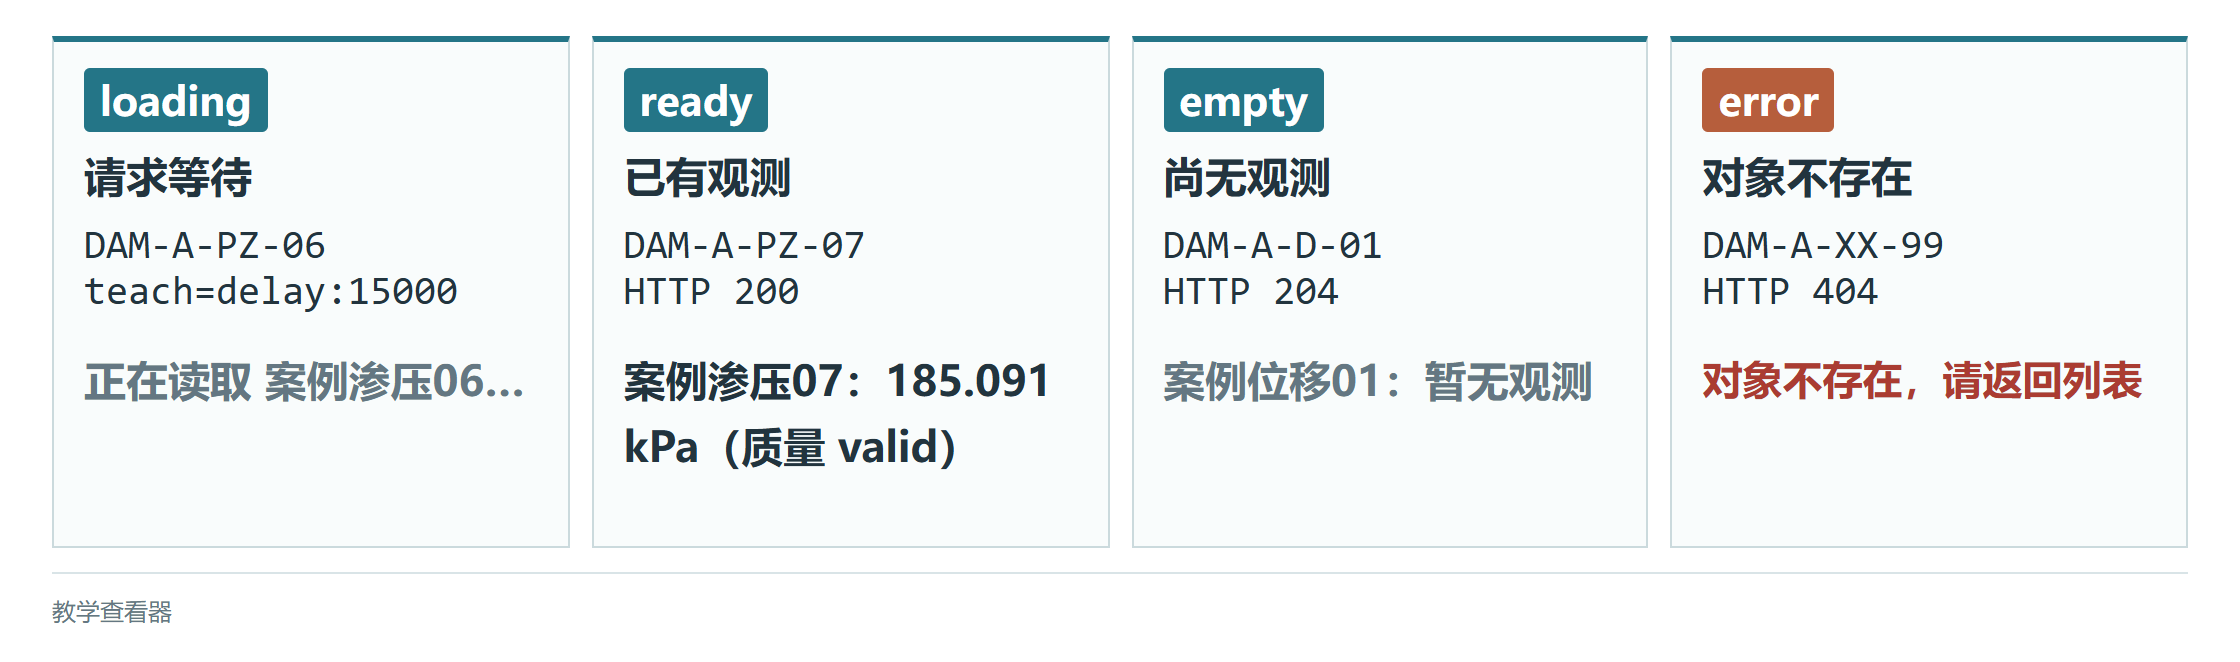
\includegraphics[width=16cm]{images/runtime/s2-four-states.png}
\caption{加载、有数据、空数据与错误状态（教学查看器，调用S2模块）}
\label{fig:ch04-state-results}
\end{figure}

\subsection{故障单元：切换测点时旧数据覆盖新数据}

\paragraph{现象}把清单\ref{lst:ch04-r1-load}改成“点击列表中的对象就读取它的最新观测”后，做如下操作：先点击 \texttt{DAM-A-PZ-07}，并让教学接口对它延迟 3 秒（请求地址加\texttt{?teach=delay:3000}）；不等结果出来，立即点击 \texttt{DAM-A-WL-01}。页面先正确显示“案例库水位01：166.837 m”，约 3 秒后却变成“案例渗压07：185.091 kPa”。值班员看着水位计的标题，读到的是渗压计的数。

\paragraph{时序}图\ref{fig:ch04-r1-race}将两次请求及页面结果放在同一时间轴上。第二次请求先返回，第一次请求随后到达。比较下方两行：无序号校验时，旧响应覆盖当前页面；校验最新请求序号后，迟到响应被丢弃，页面继续显示当前选择的对象。

\begin{figure}[htbp]
\centering
\begin{tikzpicture}[x=1cm,y=1cm,>=Stealth,font=\small,line cap=round]
  \path[use as bounding box] (0,0) rectangle (14.8,6.25);
  \tikzset{event/.style={align=center,font=\scriptsize,fill=white,inner sep=3pt},
    result/.style={align=center,rounded corners=2pt,minimum width=3.1cm,minimum height=.7cm,font=\scriptsize}}
  \node[anchor=west,font=\small\bfseries,text=PrimaryDark] at (0,5.98) {同一次切换：请求2先返回，请求1后返回};
  \draw[->,Primary!45] (1.8,5.1)--(14.3,5.1) node[right,font=\scriptsize]{时间};
  \foreach \x in {2.2,4.5,8,12.1} {\draw[Primary!30,densely dotted] (\x,1.35)--(\x,5.1);}
  \fill[Accent] (2.2,5.1) circle (2.5pt);
  \fill[Primary] (4.5,5.1) circle (2.5pt);
  \node[event,above=4pt] at (2.2,5.1) {选择 PZ-07};
  \node[event,above=4pt] at (4.5,5.1) {切换到 WL-01};
  \node[event,above=4pt,text=Primary] at (8,5.1) {响应2到达};
  \node[event,above=4pt,text=Accent!80!black] at (12.1,5.1) {响应1迟到};
  \node[anchor=west,font=\scriptsize] at (0,4.35) {请求1};
  \draw[->,Accent,line width=1.4pt] (2.2,4.35)--node[event,above]{PZ-07：延迟3秒} (12.1,4.35);
  \node[anchor=west,font=\scriptsize] at (0,3.65) {请求2};
  \draw[->,Primary,line width=1.4pt] (4.5,3.65)--node[event,above]{WL-01：先返回} (8,3.65);
  \draw[Primary!20] (0,3.16)--(14.8,3.16);
  \node[anchor=west,font=\scriptsize,align=left] at (0,2.55) {无序号校验\\每个响应都写入};
  \node[result,draw=Primary!50,fill=PrimaryLight] (good1) at (8,2.55) {显示 WL-01\\与当前选择一致};
  \node[result,draw=Accent,fill=Accent!8] (bad) at (12.1,2.55) {被 PZ-07 覆盖\\标题与数据错配};
  \draw[->,Accent,thick] (good1.east)--(bad.west);
  \node[anchor=west,font=\scriptsize,align=left] at (0,1.4) {校验最新序号\\当前序号为2};
  \node[result,draw=Primary!50,fill=PrimaryLight] (good2) at (8,1.4) {2 = 2，允许写入\\显示 WL-01};
  \node[result,draw=Primary,fill=white] (kept) at (12.1,1.4) {1 $\ne$ 2，丢弃响应\\仍显示 WL-01};
  \draw[->,Primary,thick] (good2.east)--(kept.west);
  \node[anchor=west,font=\scriptsize,text=TextGray] at (0,.45)
    {取消旧请求可节约资源；序号校验阻止已过期的结果写入页面。};
\end{tikzpicture}

\caption{迟到响应的覆盖故障与请求序号校验}
\label{fig:ch04-r1-race}
\end{figure}

\paragraph{原因}每次点击都发出一个独立的请求，每个响应回来都无条件调用\texttt{render}。页面状态与“用户当前想看哪个对象”之间没有绑定，谁最后返回谁就赢。网络慢只是让问题容易复现；只要两次请求的耗时不同，问题就存在。

\paragraph{处理方案}两道防线一起用。第一道：切换对象时用\texttt{AbortController}取消上一个请求，浏览器不再等它，被取消的\texttt{fetch}以\texttt{AbortError}拒绝，调用方要把它与服务器错误分开。第二道：给每次切换分配递增序号，响应回来时核对“我的序号是否仍是最新”，不是就丢弃。取消信号发出后，已开始处理的响应仍可能继续执行，因此写入页面前必须核对序号。清单\ref{lst:ch04-r1-race}给出完整代码，它复用清单\ref{lst:ch04-r1-load}的\texttt{loadLatest}（已接收\texttt{signal}参数）和清单\ref{lst:ch04-r1-state}的\texttt{render}；\texttt{bindList}用的是4.4.6节的事件委托。入口文件\texttt{src/lesson45/main.js}负责登录、读取对象列表、把每个对象渲染成按钮，再调用\texttt{bindList}；打开\texttt{/lesson45.html}就是这个页面。

\begin{lstlisting}[label={lst:ch04-r1-race},language=JavaScript,caption={controller.js：取消旧请求并丢弃迟到响应}]
import { loadLatest } from './detail.js';
import { State, render } from './state.js';

let sequence = 0;       // 每次切换递增；只有最新序号的响应才允许写入页面
let controller = null;  // 上一次请求的取消句柄

export async function showAsset(el, asset) {
  const mine = ++sequence;
  controller?.abort();                        // 第一道防线：通知旧请求结果不再需要
  controller = new AbortController();
  render(el, { state: State.LOADING, asset });
  try {
    const reading = await loadLatest(asset.assetId, controller.signal);
    if (mine !== sequence) return;            // 第二道防线：迟到的旧响应静默丢弃
    render(el, reading ? { state: State.READY, asset, reading }
                       : { state: State.EMPTY, asset });
  } catch (error) {
    if (error.name === 'AbortError') return;  // 被自己取消的不是故障
    if (mine !== sequence) return;
    render(el, { state: State.ERROR, asset, error });
  }
}

// 列表点击：<button data-asset-id="DAM-A-PZ-07">…</button>
export function bindList(listEl, outputEl, assets) {
  listEl.addEventListener('click', event => {
    const id = event.target.closest('button')?.dataset.assetId;
    const asset = assets.find(a => a.assetId === id);
    if (asset) showAsset(outputEl, asset);
  });
}
\end{lstlisting}

\paragraph{验证记录}重复“现象”中的操作，表\ref{tab:ch04-r1-verify}是修复前后应当观察到的差别。验收时看两处：“网络”面板中请求1 的状态是否为“已取消”，页面最终文字是否与最后点击一致。只看页面最终结果不够，网络很快的机器上修复前也可能碰巧正确。

\begin{table}[htbp]
\centering
\caption{故障单元的验证记录}
\label{tab:ch04-r1-verify}
\begin{tabular}{p{0.26\textwidth}p{0.32\textwidth}p{0.32\textwidth}}
\toprule
观察点 & 修复前 & 修复后 \\
\midrule
点击 WL-01 后的页面 & 立即显示 166.837 m & 先显示“正在读取 案例库水位01…”，再显示 166.837 m \\
约 3 秒后的页面 & 变为 185.091 kPa（错误） & 保持 166.837 m \\
“网络”面板中请求1 & 200，耗时约 3 s & 状态“已取消”（canceled） \\
控制台 & 无输出 & 无输出：AbortError 被识别为正常路径，不打印 \\
再点击一次 PZ-07 & 显示 185.091 kPa & 显示 185.091 kPa（序号已更新，新请求正常写入） \\
\bottomrule
\end{tabular}
\end{table}

\paragraph{延伸}同一个模式在本书后面反复出现：4.7 节 Pinia 仓库的\texttt{loadLatest}用同样的序号校验，否则切换测点时读数会闪回；7.4 节切换三维对象时，详情面板也不能显示上一个对象的观测；第8章预警确认属于写操作，取消请求并不能撤销服务端已完成的确认，那里要靠幂等键而不是序号。

图\ref{fig:ch04-switch-results}记录先选渗压点、再选水位点的请求次序。旧请求取消后，页面保持最后选中的水位对象。

\begin{figure}[htbp]
\centering
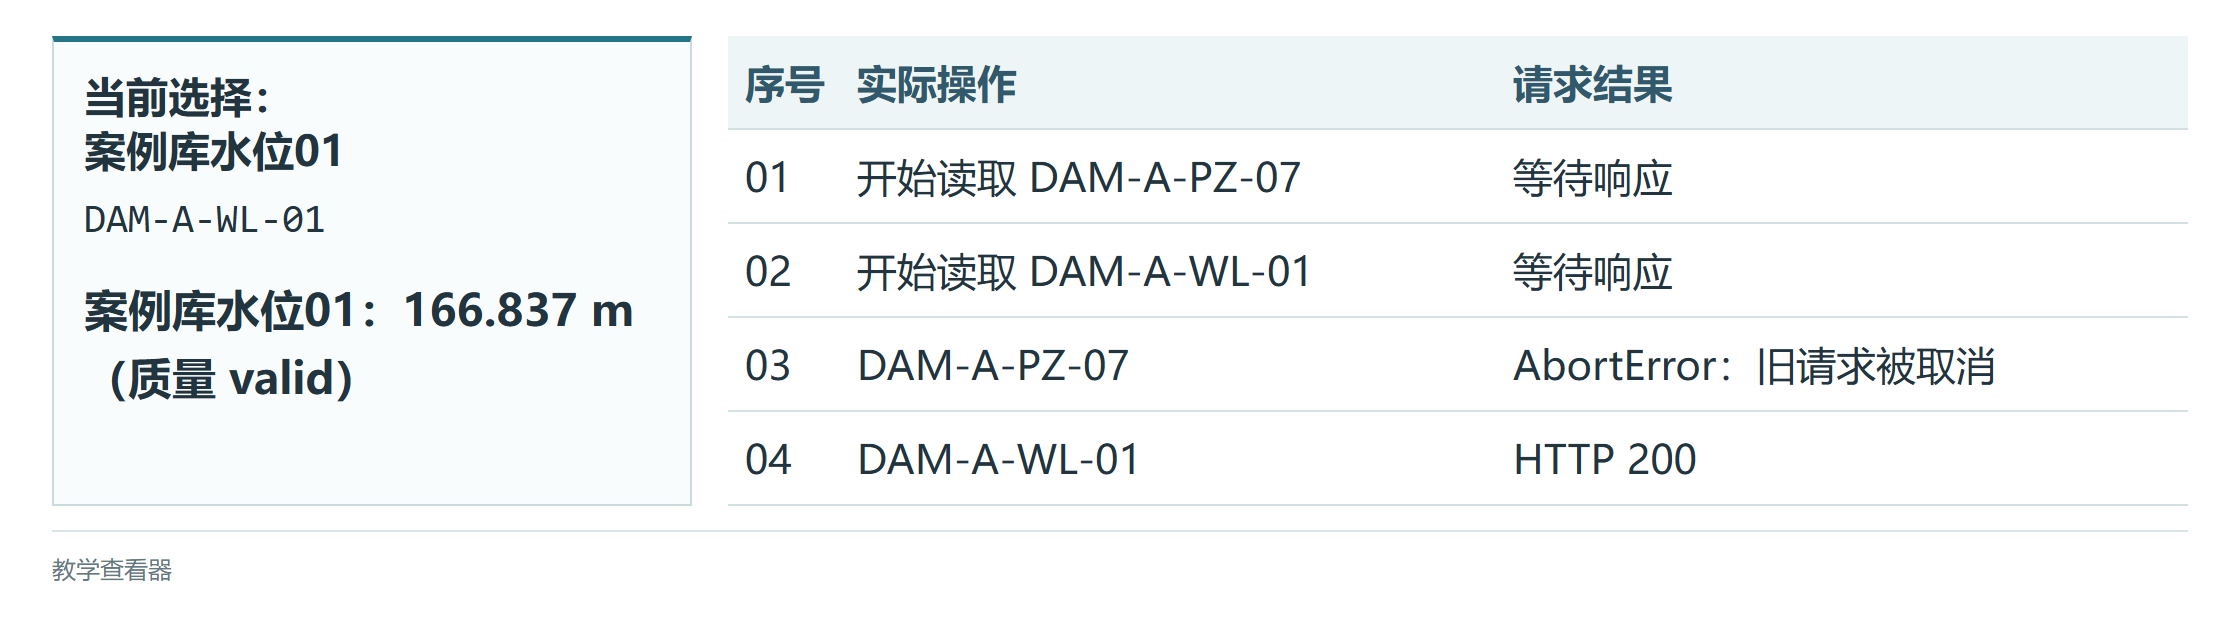
\includegraphics[width=16cm]{images/runtime/s2-switch-trace.png}
\caption{切换测点后的取消记录与最终页面（教学查看器，调用S2模块）}
\label{fig:ch04-switch-results}
\end{figure}

\subsection{request.js：JWT、401 与超时的统一入口}

清单\ref{lst:ch04-r1-load}把令牌放在模块变量里，刷新页面就没了，\texttt{getJson}也只有这一个页面能用。4.6节以后的 Vue 页面共用一个请求模块\texttt{src/api/request.js}。令牌是第5章后端签发的 JWT：一段带签名和有效期的字符串，后端凭它确认请求者是谁。登录成功后前端保存令牌，后续每个请求在\texttt{Authorization: Bearer <token>}头里带上它；收到 401 说明令牌失效，清除令牌并跳转登录页，不拿旧令牌重试。

教学示例把令牌放入\texttt{sessionStorage}，关闭标签页后令牌消失；代价是页面一旦被注入恶意脚本（4.4.4节的 XSS），脚本可以读走它。生产系统要结合内容安全策略、短有效期和 HttpOnly Cookie 方案评估。签名密钥只存在于后端，任何以\texttt{VITE\_}开头的前端变量都会被打包进浏览器能下载的文件，不能存放密钥。

清单\ref{lst:ch04-a45-request}就是配套工程的\texttt{src/api/request.js}。它统一处理令牌注入、JSON 头、204 空响应、超时和 401 跳转；超时的做法是用\texttt{setTimeout}在 10 秒后调用\texttt{controller.abort()}，与4.5.4节取消旧请求用的是同一个机制。请求函数只负责传输和认证，页面层根据错误代码决定显示“重新登录”“稍后重试”还是“检查测站输入”。

\begin{lstlisting}[label={lst:ch04-a45-request},language=JavaScript,caption={request.js：令牌注入、401 跳转与超时}]
const API_BASE = import.meta.env.VITE_API_ORIGIN ?? '';   // 契约路径已含 /api 前缀
const DEFAULT_TIMEOUT = 10_000;
// 令牌键名是前端各模块的共同契约：请求封装、路由守卫、
// 登录页都从这里导入，避免"登录成功却处处 401"的隐蔽错误
export const TOKEN_KEY = 'access_token';

function accessToken() {
  return sessionStorage.getItem(TOKEN_KEY);
}

export async function request(path, options = {}) {
  const controller = new AbortController();
  const timeoutId = setTimeout(
    () => controller.abort(), options.timeoutMs ?? DEFAULT_TIMEOUT
  );
  const headers = new Headers(options.headers);
  headers.set('Accept', 'application/json');
  if (options.body && !headers.has('Content-Type')) {
    headers.set('Content-Type', 'application/json');
  }
  const token = accessToken();
  if (token) headers.set('Authorization', `Bearer ${token}`);

  try {
    const response = await fetch(`${API_BASE}${path}`, {
      ...options, headers, signal: controller.signal
    });
    if (response.status === 401 && !path.startsWith('/api/auth/')) {
      // 业务请求的 401 才代表登录态失效；
      // 登录接口自身的 401 是"密码错误"，交回页面层提示
      sessionStorage.removeItem(TOKEN_KEY);
      const redirect = encodeURIComponent(location.pathname + location.search);
      location.assign(`/login?redirect=${redirect}`);
      throw new Error('UNAUTHORIZED');
    }
    if (!response.ok) throw new Error(`HTTP_${response.status}`);
    if (response.status === 204) return null;
    return response.json();
  } catch (error) {
    if (error.name === 'AbortError') {
      throw new Error('REQUEST_TIMEOUT', { cause: error });
    }
    throw error;
  } finally {
    clearTimeout(timeoutId);
  }
}
\end{lstlisting}

\subsection{Vite 代理与环境变量}

Vite 是本章使用的前端开发工具：\texttt{npm run dev}启动一个开发服务器，修改源文件后页面自动刷新；\texttt{npm run build}把源文件打包成可部署的静态文件。开发时页面由 Vite 的 5173 端口提供，后端在 8080 端口；协议、域名、端口有一项不同就算“不同源”，浏览器默认不允许页面脚本读取不同源接口的响应，这就是跨域限制。Vite 的\texttt{server.proxy}让开发服务器代为转发：浏览器请求同源的\texttt{/api/...}，Vite 在服务器一侧转给 8080。生产环境由 Nginx 或网关做同样的路径转发。代理只解决开发时的跨域，与后端认证无关。

只有以\texttt{VITE\_}开头的环境变量会暴露给浏览器代码（通过\texttt{import.meta.env}读取），它们的值在构建时被直接替换进 JavaScript 文件，所以只能放 API 基地址、功能开关这类公开信息。清单\ref{lst:ch04-a45-vite}是带代理的\texttt{vite.config.js}：\texttt{loadEnv}按运行模式读取\texttt{.env}文件，代理目标缺省指向本机 8080。修改配置后重启\texttt{npm run dev}，在“网络”面板里看到\texttt{/api/assets}的请求地址仍是 5173 端口，而教学接口的终端里出现了对应的访问记录，说明代理生效。

\begin{lstlisting}[label={lst:ch04-a45-vite},language=JavaScript,caption={Vite 5 的 server.proxy 与 import.meta.env}]
import { defineConfig, loadEnv } from 'vite';
import vue from '@vitejs/plugin-vue';

export default defineConfig(({ mode }) => {
  const env = loadEnv(mode, process.cwd(), 'VITE_');
  return {
    plugins: [vue()],
    server: {
      proxy: {
        '/api': {
          target: env.VITE_PROXY_TARGET ?? 'http://localhost:8080',
          changeOrigin: true,
          secure: false
        }
      }
    },
    define: {
      __BUILD_MODE__: JSON.stringify(mode)
    }
  };
});
\end{lstlisting}

\subsection{登录与受保护接口的前后端联调}

一次受保护的请求要过几道关。登录接口返回访问令牌；\texttt{request.js}在每个请求里注入 Bearer 头；后端的 JWT 过滤器验证签名和有效期，通过后把用户身份放进安全上下文；授权规则再决定这个身份能不能调用目标接口。图\ref{fig:ch04-jwt-integration}把这条链路与两个失败分支画在一起，后端各环节的实现见第5章。

\begin{figure}[htbp]
\centering
\begin{tikzpicture}[>=Stealth,thick,node distance=0.55cm and 0.45cm]
  \tikzset{authstage/.style={draw=Primary,rounded corners=2pt,minimum width=2.2cm,minimum height=.75cm,align=center,fill=PrimaryLight,text=PrimaryDark,font=\scriptsize},
    fail/.style={draw=Accent,rounded corners=2pt,minimum width=2.2cm,minimum height=.65cm,align=center,fill=white,text=PrimaryDark,font=\scriptsize}}
  \node[authstage] (login) {登录成功\\保存accessToken};
  \node[authstage,right=of login] (request) {request.js\\注入 Bearer};
  \node[authstage,right=of request] (filter) {JWT过滤器\\验签/过期/jti};
  \node[authstage,right=of filter] (security) {URL/方法授权\\读取安全上下文};
  \node[authstage,right=of security] (api) {Controller\\返回数据};
  \node[fail,below=of filter] (auth401) {401\\清理令牌并登录};
  \node[fail,below=of security] (auth403) {403\\显示权限不足};
  \draw[->,draw=Primary] (login)--(request);
  \draw[->,draw=Primary] (request)--(filter);
  \draw[->,draw=Primary] (filter)--(security);
  \draw[->,draw=Primary] (security)--(api);
  \draw[->,draw=Accent] (filter) -- node[right,font=\scriptsize]{失效} (auth401);
  \draw[->,draw=Accent] (security) -- node[right,font=\scriptsize]{无权限} (auth403);
\end{tikzpicture}
\caption{前端登录、JWT过滤器与受保护接口的联调链路}
\label{fig:ch04-jwt-integration}
\end{figure}

联调时把状态码和界面行为一一对应。401 表示“不知道你是谁”：清理本地令牌，带着原始路径跳到登录页。403 表示“知道你是谁，但你无权做这件事”：留在当前页面显示无权提示，跳回登录页没有意义。404 说明测站不存在；400 要按\texttt{field}把错误写回表单。前端不能把“没有令牌”和“令牌已过期”都显示成空列表，否则值班员只能靠反复刷新来猜系统状态。登录请求的字段名、令牌字段和失败错误码以表\ref{tab:api-contract}为准；令牌的键名由所有模块从清单\ref{lst:ch04-a45-request}导入同一个\texttt{TOKEN\_KEY}常量，键名对不上是“登录成功却处处 401”的常见原因。登录函数的写法已见清单\ref{lst:ch04-r1-load}，Vue 登录页见4.7.1节。

联调中另有三类问题容易误判。一是时钟：浏览器与服务端时钟相差过大，刚签发的令牌会被判为尚未生效或已过期，这时应记录服务端时间与令牌里的\texttt{iat}、\texttt{exp}，而不是放宽过期校验。二是跨域报错：先确认请求是否绕过了代理（地址里出现了 8080），再考虑后端的跨域配置；允许任意来源不能解决认证问题，还会扩大令牌泄露面。三是重试：网络超时后可以重试 GET，创建处置单这类 POST 必须带幂等键（第8章）；多个并发请求同时收到 401 时，只清理和跳转一次。

\begin{table}[htbp]
\centering
\caption{前后端认证联调的检查记录}
\label{tab:ch04-auth-contract}
\begin{tabular}{p{0.22\textwidth}p{0.30\textwidth}p{0.34\textwidth}}
\toprule
检查点 & 浏览器证据 & 服务端证据 \\
\midrule
登录成功 & POST 返回 200，响应含 accessToken，未把密码写入日志 & issuer、subject、type 和 exp 校验通过 \\
访问列表 & 请求带 Authorization，响应 200 或明确的 401/403 & 过滤器写入 SecurityContext，权限方法给出决策 \\
令牌过期 & 收到一次 401，令牌被清理并回到原路径 & 记录 jti、失败原因和请求追踪 ID，不记录完整令牌 \\
网络异常 & 超时显示重试，幂等请求才自动重试 & 网关和应用日志能按追踪 ID 对齐时间线 \\
\bottomrule
\end{tabular}
\end{table}

每次联调按表\ref{tab:ch04-auth-contract}逐行记录请求时间、状态码和去掉令牌后的响应摘要。有了这份记录，前后端对“到底通没通”的判断依据是同一组可以重放的请求。

\subsection{拓展：认证契约测试与故障复盘}

能登录只是第一步，难点在多个请求同时发生、页面刷新和网络抖动时，页面是否仍然按同一套规则反应。4.5.4 节的竞态覆盖可以写成自动化测试：让第一个模拟请求延迟 200 毫秒、第二个只延迟 20 毫秒，连续调用两次\texttt{showAsset}，断言页面最终文字属于第二个对象、第一个请求收到取消信号。配套工程的\texttt{tests/lesson45.test.js}就是这样写的，在\texttt{frontend/}目录执行\texttt{npm test}运行。

错误提示要区分能不能通过重试恢复。表\ref{tab:ch04-auth-errors}按状态码列出含义和前端动作：401 重试同一个请求没有意义；403 自动重试只会制造日志噪声；409 表示版本或幂等键冲突，要重新读取后由人确认；429 和 503 可以重试，但要遵守服务端\texttt{Retry-After}头或逐次加长间隔，并设最大次数。前端读取稳定的\texttt{code}字段，不从错误文本里猜状态。

\begin{table}[htbp]
\centering
\caption{认证及接口错误的前端处理矩阵}
\label{tab:ch04-auth-errors}
\begin{tabular}{p{0.17\textwidth}p{0.28\textwidth}p{0.38\textwidth}}
\toprule
状态 & 业务含义 & 前端动作与验收证据 \\
\midrule
401 & 未登录或访问令牌失效 & 清理令牌、保留原路径、只发起一次登录跳转；记录脱敏 traceId \\
403 & 已识别身份但权限不足 & 停留当前页面，展示所需权限和申请入口；不得循环登录 \\
404 & 测站或事件不存在 & 显示资源不存在并提供返回列表；不把空对象当作零值 \\
409 & 版本或幂等键冲突 & 重新读取资源并提示人工确认；保留冲突双方版本号 \\
429/503 & 限流或服务暂不可用 & 按 Retry-After 或退避重试，超过上限后提供手动重试 \\
\bottomrule
\end{tabular}
\end{table}

表中每一行都可以改写成一个端到端测试用例，包含初始路由、是否已有令牌、请求次数、最终 URL 和页面可见文案；涉及权限的用例固定测试账号的角色。用教学接口的\texttt{teach=}参数可以依次制造 401、400、503 和延迟，每种故障注入后检查四件事：页面是否仍可操作，是否产生重复请求，是否保存了原路径，是否把故障与正常读数、空结果明确区分。

接口字段升级、跨域预检、令牌存储方式的取舍、认证性能和联调记录归档等内容见附录C的\ref{app:ext-fe-auth}节。

\subsection{拓展：事件循环与任务调度}

4.1节提到 JavaScript 在一个线程里依次处理任务，这里说明“依次”的规则。当前同步代码执行完后，事件循环先清空微任务队列，再从任务队列取下一个任务（也叫宏任务）。网络回调、定时器和用户输入进入任务队列；\texttt{Promise.then}、\texttt{await}之后的代码和\texttt{queueMicrotask}的回调进入微任务队列。所以清单\ref{lst:ch04-a45-event-loop}的输出顺序与书写顺序不同：两条同步输出在前，两条微任务其次，\texttt{setTimeout}即使延迟为 0 也排在最后。

微任务适合做同一轮里的短小收尾，例如把多个状态变化合并后再通知界面。微任务执行期间浏览器不能绘制也不能响应输入，长时间运行的微任务会让页面卡住。处理大量测点时，把计算分批放进任务队列或交给 Web Worker（浏览器提供的后台线程）。

\begin{lstlisting}[label={lst:ch04-a45-event-loop},language=JavaScript,caption={事件循环中的同步、微任务与宏任务}]
console.log('同步：开始读取');

setTimeout(() => console.log('宏任务：定时刷新'), 0);
queueMicrotask(() => console.log('微任务：合并状态'));
Promise.resolve().then(() => console.log('微任务：更新摘要'));

console.log('同步：结束读取');
// 典型顺序：开始、结束、合并状态、更新摘要、定时刷新
\end{lstlisting}

\subsection{自测与下一步}

\begin{enumerate}
\item 把清单\ref{lst:ch04-r1-load}中最后一行的对象换成 \texttt{DAM-A-RF-01}，页面显示什么？再把地址改成 \texttt{DAM-A-RF-99}，页面应显示什么、“网络”面板的状态码是多少？（参考：雨量计的最新观测与单位 mm；404 与“对象不存在，请返回列表”。）
\item 只保留清单\ref{lst:ch04-r1-race}的序号校验、删去\texttt{AbortController}，故障单元的验证记录哪几行会变？（参考：页面结果仍正确，但请求1 不再显示“已取消”，仍会占用 3 秒带宽并返回 200。）
\item 教学接口对\texttt{/api/assets}返回\texttt{?teach=empty}时，列表页应当显示什么？如果显示“服务暂时不可用”，说明状态模型哪里错了？（参考：空数组是 empty 而非 error；把\texttt{[]}当成失败是把“没有数据”和“拿不到数据”混为一谈。）
\end{enumerate}

4.6 节用 Vue 组件承接同一份状态模型；4.7 节把\texttt{showAsset}的序号校验搬进 Pinia 仓库；4.8 节给出 S1、S2 两个阶段的验收检查单。完成第5章的存储、统一异常处理和认证后，先停掉教学接口并启动完整的 Spring Boot 后端，再执行契约检查，核对页面的四种状态。

\section{Vue 3组件化开发}

\paragraph{本节层次}核心：4.6.1、4.6.2；指导实践：4.6.3、4.6.4。

\paragraph{进入本节所需知识}读过4.4节与4.5节核心内容，写过“数据变了就手动改 DOM”的代码；配套工程\texttt{frontend/}已执行过\texttt{npm ci}。

4.5节的\texttt{render}函数每次状态变化都要自己找到节点、改写文字。页面上只有一行输出时这不难；仪表盘同时有曲线、表格和预警标识时，“哪个数据变了要改哪几个节点”很快就理不清。Vue 换了一种写法：你在模板里声明“界面长什么样、各处显示哪个状态”，把状态存进 Vue 提供的响应式变量，之后只改变量，DOM 由框架同步。界面仍要遵守反馈及时、操作一致这些基本设计原则\cite{norman2013}。

一个 Vue 组件写在一个\texttt{.vue}文件里，叫单文件组件（SFC）：\texttt{<script setup>}块写状态和逻辑，\texttt{<template>}块写模板，可选的\texttt{<style>}块写样式。本章使用 Vue 3.4+ 的组合式 API，响应式系统的完整说明见官方文档\cite{vueDocs}。清单\ref{lst:ch04-vue-component}是一个完整的测站卡片组件。\texttt{defineProps}声明父组件可以传进来的数据（props）及其类型；\texttt{computed}定义一个由其他状态算出来的值，依赖变了自动重算；模板里的双花括号显示一个表达式的值，\texttt{:class}把属性绑定到表达式，\texttt{@click}登记点击处理；\texttt{emit}向父组件发出一个事件。数据由父到子经 props 向下传，子组件通过事件向上通知，这是 Vue 组件之间的基本约定。

把清单保存为\texttt{src/components/AssetCard.vue}，在任一页面组件里\texttt{import AssetCard from './components/AssetCard.vue'}，模板中写\texttt{<AssetCard display-name="案例库水位01" :value="166.84" />}，\texttt{npm run dev}后页面出现一张带\texttt{station-card--warning}类的卡片；把数值改成 165.12，类名变为\texttt{station-card--normal}。

\begin{lstlisting}[label={lst:ch04-vue-component},language=Vue,caption={测站卡片组合式组件}]
<script setup>
import { computed } from 'vue'
const props = defineProps({
  displayName: { type: String, required: true },
  value: { type: Number, required: true },
  unit: { type: String, default: 'm' }
})
const emit = defineEmits(['open-detail'])
// 165.5 m 是案例水库汛限水位（8.1 节参数表）；真实阈值应来自后端
const status = computed(() => props.value >= 165.5 ? 'warning' : 'normal')
</script>

<template>
  <article :class="['station-card', `station-card--${status}`]">
    <h3>{{ displayName }}</h3>
    <p>当前值：{{ value.toFixed(2) }} {{ unit }}</p>
    <button type="button" @click="emit('open-detail')">查看详情</button>
  </article>
</template>
\end{lstlisting}

\subsection{Vue 3.4 组合式 API 与响应式状态}

普通变量改了值，Vue 并不知道；要让界面跟着变，状态必须放进响应式容器。\texttt{ref}包住一个值，在脚本里通过\texttt{.value}读写，在模板里直接写变量名，Vue 自动取出里面的值。\texttt{reactive}把一个对象变成响应式的，直接读写属性即可；不能把整个对象重新赋值，那样会丢掉响应式。常见分工是：表单的一组字段用\texttt{reactive}，加载标志、选中的编码、会被接口结果整体替换的数组用\texttt{ref}。

从已有状态算出来的结果用\texttt{computed}，例如筛选后的列表；它会缓存，依赖不变就不重算。状态变化时要“做一件事”（发请求、写存储、打日志）用\texttt{watch}，它监听一个明确的来源；\texttt{watchEffect}自动追踪函数里用到的所有响应式状态，适合小范围联动。表\ref{tab:ch04-a46-reactivity-choice}把五个 API 的用途和常见错误放在一起。判断方法很简单：结果能由现有状态纯计算得到，用\texttt{computed}；要访问网络或修改外部东西，用\texttt{watch}。\texttt{computed}里出现了\texttt{fetch}，或者\texttt{watch}里只是拼了个字符串，都说明用错了。

\begin{table}[H]
\centering
\caption{Vue 响应式 API 的职责边界与验收问题}
\label{tab:ch04-a46-reactivity-choice}
\begin{tabular}{p{2.3cm}p{3.5cm}p{4.8cm}}
\toprule
API & 适合表达的内容 & 代码评审时的核对问题 \\
\midrule
\texttt{ref} & 基本值、可整体替换的对象 & 是否在 JavaScript 中正确使用\texttt{.value}，模板是否依赖自动解包 \\
\texttt{reactive} & 表单、稳定结构的对象和数组 & 是否把代理对象整体替换，是否把深层可变状态暴露给子组件 \\
\texttt{computed} & 过滤、排序、格式化等纯派生值 & 函数是否无网络请求和写操作，依赖是否完整 \\
\texttt{watch} & 具有明确来源的异步或外部副作用 & 是否处理竞态、错误和清理，是否设定合理的\texttt{flush}时机 \\
\texttt{watchEffect} & 少量依赖的同步联动 & 自动收集的依赖是否稳定，是否会因隐式访问造成重复执行 \\
\bottomrule
\end{tabular}
\end{table}

清单\ref{lst:ch04-a46-reactivity}是测站筛选页\texttt{AssetFilterPage.vue}的脚本部分，数据先写死两条，4.6.4节再换成接口。对象列表的字段取自表\ref{tab:api-contract}。\texttt{watch}在选中编码变化时执行，\texttt{watchEffect}在筛选结果数量变化时执行。这一段还没有模板，页面上没有输入框；先保存并打开控制台，能看到\texttt{watchEffect}首次执行时打印的“筛选数量 2”。补上4.6.2节的模板以后，在页面上输入关键字，就能看到这个数字随输入变化。

\begin{lstlisting}[label={lst:ch04-a46-reactivity},language=Vue,caption={AssetFilterPage.vue 的脚本：响应式状态、计算属性与监听器}]
<script setup>
import { computed, reactive, ref, watch, watchEffect } from 'vue';

const selectedId = ref('DAM-A-PZ-07');
const form = reactive({ keyword: '', assetType: '' });
const assets = ref([
  { assetId: 'DAM-A-WL-01', displayName: '案例库水位01', assetType: '库水位', unit: 'm' },
  { assetId: 'DAM-A-PZ-07', displayName: '案例渗压07', assetType: '渗压', unit: 'kPa' }
]);
const visibleAssets = computed(() => assets.value.filter(asset => {
  const match = asset.displayName.includes(form.keyword);
  return match && (form.assetType === '' || asset.assetType === form.assetType);
}));

watch(selectedId, id => console.log('重新加载测站', id));
watchEffect(() => console.log('筛选数量', visibleAssets.value.length));
</script>
\end{lstlisting}

阈值计算和数据质量判定由后端给出结论，前端的响应式状态只管界面；展示读数时保留测点编号、采样时间和质量码，值班员才能追溯。

\subsection{模板指令与组件通信}

模板里以\texttt{v-}开头的属性叫指令，它们把状态映射成 HTML。\texttt{v-if}按条件创建或销毁节点，适合权限区域、错误提示这类不常切换的内容；\texttt{v-show}保留节点、只切换\texttt{display}，适合反复开合的筛选面板。\texttt{v-for}按数组渲染一组节点，必须配一个稳定且唯一的\texttt{:key}，用对象编码，不用数组下标：列表筛选或排序后，Vue 靠 key 判断哪一行是哪一行，用下标会把旧行的焦点和输入内容错配给另一个测站。\texttt{v-model}让输入控件与状态双向同步，修饰符\texttt{.trim}去掉首尾空白；\texttt{v-bind}（简写为冒号）绑定属性，\texttt{v-on}（简写为\texttt{@}）绑定事件。

清单\ref{lst:ch04-a46-directives}是同一个文件的模板部分，接在清单\ref{lst:ch04-a46-reactivity}的\texttt{</script>}之后。模板只声明关系，筛选逻辑留在\texttt{computed}里。在下拉框里选“渗压”，列表只剩一行；点击某一行的按钮，“当前”标记移到这一行，控制台同时打印\texttt{watch}的输出。

\begin{lstlisting}[label={lst:ch04-a46-directives},language=Vue,caption={AssetFilterPage.vue 的模板：指令与稳定 key}]
<template>
  <label>
    关键字
    <input v-model.trim="form.keyword" type="search">
  </label>
  <label>
    类型
    <select v-model="form.assetType">
      <option value="">全部</option>
      <option>库水位</option>
      <option>渗压</option>
    </select>
  </label>
  <p v-show="form.keyword === ''" class="hint">输入名称中的任意几个字即可筛选</p>
  <ul>
    <li v-for="asset in visibleAssets" :key="asset.assetId">
      <button type="button" v-bind:aria-label="`打开${asset.displayName}`"
              v-on:click="selectedId = asset.assetId">
        {{ asset.displayName }}（{{ asset.unit }}）
      </button>
      <span v-if="asset.assetId === selectedId" class="current">当前</span>
    </li>
  </ul>
</template>
\end{lstlisting}

组件之间有四种传递方式。props 由父到子传只读数据，子组件不修改它；emit 由子到父报告用户动作，事件名描述意图（\texttt{select}、\texttt{retry}），参数只带业务主键。slot（插槽）让父组件往子组件里塞一段自己的模板，例如替换卡片的操作区，而不必复制整张卡片。provide/inject 跨越多层组件传递只读配置，例如兜底单位、主题和请求客户端；会变化的业务状态不走这条路，交给4.7节的 Pinia，状态归谁管才看得清。

清单\ref{lst:ch04-a46-communication}在清单\ref{lst:ch04-vue-component}的卡片上加了后两种方式：\texttt{<slot name="actions">}里的按钮是默认内容，父组件提供了同名插槽就用父组件的；\texttt{inject}取得上层\texttt{provide}的兜底单位，第二个参数是没人提供时的默认值。父组件用\texttt{readonly}包住提供的值，子组件无法改动它。测试这个组件时从约定出发：给定 props 检查渲染出的标题和单位；点击按钮后断言发出的事件名和参数；替换插槽后确认按钮仍有可访问名称。

\begin{lstlisting}[label={lst:ch04-a46-communication},language=Vue,caption={Vue props、emit、slot 与 provide/inject}]
<!-- AssetCard.vue -->
<script setup>
import { inject } from 'vue';
const props = defineProps({ asset: { type: Object, required: true } });
const emit = defineEmits(['select']);
const fallbackUnit = inject('fallbackUnit', 'm');
</script>
<template>
  <article>
    <h3>{{ props.asset.displayName }}</h3>
    <p>当前值：{{ props.asset.value }} {{ props.asset.unit ?? fallbackUnit }}</p>
    <slot name="actions">
      <button type="button" @click="emit('select', props.asset.assetId)">查看</button>
    </slot>
  </article>
</template>

<!-- AssetPanel.vue 的 script setup 片段 -->
<script setup>
import { provide, readonly, ref } from 'vue';
const fallbackUnit = ref('m');   // 对象自身没有单位时的兜底
provide('fallbackUnit', readonly(fallbackUnit));
</script>
\end{lstlisting}

\subsection{生命周期与资源清理}

组件从创建到销毁经过几个固定时刻，Vue 在这些时刻调用你登记的函数，叫生命周期钩子。图\ref{fig:vue-lifecycle}画出组合式 API 的钩子顺序：\texttt{setup}建立状态，挂载后调用\texttt{onMounted}，此时模板已经变成真实的 DOM；响应式状态变化引起的 DOM 更新可以发生零次或多次；组件离开页面时调用\texttt{onUnmounted}。Vue 3 的卸载钩子是\texttt{onBeforeUnmount}和\texttt{onUnmounted}，网上不少旧资料里的\texttt{beforeDestroy}、\texttt{destroyed}是 Vue 2 的名字。

\begin{figure}[htbp]
\centering
\begin{tikzpicture}[>=Stealth,
  life/.style={draw=Primary,rounded corners=2pt,fill=PrimaryLight,text=PrimaryDark,text width=4.1cm,minimum height=.65cm,align=center,font=\small}]
  \node[life] (setup) at (0,0) {setup：建立组件状态};
  \node[life] (beforemount) at (0,-1.1) {onBeforeMount};
  \node[life] (mounted) at (0,-2.2) {onMounted};
  \node[life] (active) at (0,-3.3) {组件运行中};
  \node[life] (unmount) at (0,-4.7) {onBeforeUnmount};
  \node[life] (unmounted) at (0,-5.8) {onUnmounted};
  \node[life] (update) at (6.2,-3.3) {onBeforeUpdate\\DOM更新\\onUpdated};
  \draw[->,Primary,thick] (setup)--(beforemount);
  \draw[->,Primary,thick] (beforemount)--(mounted);
  \draw[->,Primary,thick] (mounted)--(active);
  \draw[->,Primary,thick] (active)--node[left,font=\scriptsize]{卸载}(unmount);
  \draw[->,Primary,thick] (unmount)--(unmounted);
  \draw[->,Primary,thick] (active.east)--node[above,align=center,font=\scriptsize]{状态变化\\触发更新}(update.west);
  \draw[->,Accent,thick] (update.south)--(6.2,-4.25)--(2.8,-4.25)--(2.8,-3.55)--(active.south east);
  \node[font=\scriptsize,text=TextGray,align=center] at (6.2,-1.95) {更新可发生零次或多次};
\end{tikzpicture}
\caption{Vue 3组件生命周期与可重复的更新分支}
\label{fig:vue-lifecycle}
\end{figure}

定时刷新、WebSocket 连接、图表和三维场景实例都在\texttt{onMounted}里建立、在\texttt{onUnmounted}里释放。忘记释放时，值班员在页面之间来回切换几次，后台就留下好几个还在发请求的定时器，内存也一直涨。清单\ref{lst:ch04-a46-lifecycle}是一个每 30 秒刷新一次的组件：\texttt{onMounted}保存定时器句柄，\texttt{onUnmounted}用这个句柄清除定时器，并通过\texttt{AbortController}取消还没返回的请求。验证方法：挂载组件后在“网络”面板看到每 30 秒一条请求；切到别的页面后请求停止；再切回来，仍然只有一路请求。

\begin{lstlisting}[label={lst:ch04-a46-lifecycle},language=Vue,caption={onMounted 与 onUnmounted 的清理模式}]
<script setup>
import { onMounted, onUnmounted, ref } from 'vue';

const latest = ref(null);
const controller = new AbortController();
let timerId;

async function refresh() {
  const response = await fetch('/api/assets/DAM-A-PZ-07/readings/latest', {
    signal: controller.signal
  });
  if (response.ok) latest.value = await response.json();
}

onMounted(() => {
  refresh();
  timerId = window.setInterval(refresh, 30_000);
});
onUnmounted(() => {
  window.clearInterval(timerId);
  controller.abort();
});
</script>
\end{lstlisting}

刷新间隔由业务允许的延迟决定：案例水库的实时读数允许三十秒延迟，就用三十秒。上一次请求还没回来时不要再发一次，可以用加载标志挡住，或者像4.5.4节那样取消旧请求；标签页转入后台时可以暂停刷新，回到前台立即拉取一次。

\subsection{测站列表筛选页：从 SFC 到组件拆分}

现在把4.6.1和4.6.2节的\texttt{AssetFilterPage.vue}补成可交付的页面：数据来自接口，有加载中、空结果和正常三种显示，列表行拆成独立组件。父组件负责取数、保存筛选条件和计算可见集合；行组件只管一行的显示和发出选择事件，以后可以在地图侧栏复用。

清单\ref{lst:ch04-a46-station-row}是行组件\texttt{AssetRow.vue}。清单\ref{lst:ch04-a46-station-filter}只列出\texttt{AssetFilterPage.vue}相对前两份清单的改动：写死的数组换成空数组，挂载后用清单\ref{lst:ch04-a45-request}的\texttt{request}读取\texttt{/api/assets}；模板里的\texttt{<ul>}换成三个分支。运行前启动教学接口和开发服务器并先登录；页面先显示“正在加载测站……”，随后列出 28 个对象；关键字输入“不存在”，显示“没有符合条件的测站”。

\begin{lstlisting}[label={lst:ch04-a46-station-row},language=Vue,caption={测站列表行组件 AssetRow.vue}]
<script setup>
defineProps({
  asset: { type: Object, required: true },
  selected: { type: Boolean, default: false }
});
const emit = defineEmits(['select']);
</script>

<template>
  <li :class="{ selected }">
    <button type="button" @click="emit('select', asset.assetId)">
      <strong>{{ asset.displayName }}</strong>
      <span>{{ asset.assetType }}，单位 {{ asset.unit }}</span>
      <span v-if="selected" class="current">当前</span>
    </button>
  </li>
</template>
\end{lstlisting}

\begin{lstlisting}[label={lst:ch04-a46-station-filter},language=Vue,caption={AssetFilterPage.vue 的改动：接口取数、三种显示与行组件}]
<script setup>
import { computed, onMounted, reactive, ref } from 'vue';
import AssetRow from './AssetRow.vue';
import { request } from '../api/request.js';

const assets = ref([]);                 // 写死的两条数据改为空数组
const loading = ref(false);
// selectedId、form、visibleAssets 与 4.6.1 节的脚本清单相同

async function loadAssets() {
  loading.value = true;
  try {
    assets.value = await request('/api/assets');
  } finally {
    loading.value = false;
  }
}
function selectAsset(id) { selectedId.value = id; }
onMounted(loadAssets);
</script>

<template>
  <!-- 两个 <label> 与 4.6.2 节的模板清单相同 -->
  <p v-if="loading" role="status">正在加载测站……</p>
  <p v-else-if="visibleAssets.length === 0">没有符合条件的测站</p>
  <ul v-else>
    <AssetRow v-for="asset in visibleAssets" :key="asset.assetId"
              :asset="asset" :selected="asset.assetId === selectedId"
              @select="selectAsset" />
  </ul>
</template>
\end{lstlisting}

这个页面还缺错误状态：\texttt{request}失败时\texttt{loadAssets}会抛出异常，页面却停在空列表上。参照4.5.3节的四种状态补一个\texttt{error}变量和对应的\texttt{v-else-if}分支，再用\texttt{?teach=error}验证，是本小节的练习。交付前按四个方面各检查一遍：数据（字段、单位、时间格式和质量码是否与契约一致）；交互（关键字、类型筛选、键盘选择）；错误（加载失败、令牌过期、超时、空结果）；可访问性（标题层级、表单标签、焦点可见、\texttt{role="status"}的加载提示能被读屏软件读到）。每一项写出输入和预期输出。

\section{Vue Router与Pinia应用组织}

\paragraph{本节层次}指导实践：4.7.1、4.7.2、4.7.3、4.7.4。

\paragraph{进入本节所需知识}读过4.6节核心内容；本节复用4.5.5节的\texttt{request.js}，运行时需要教学接口和\texttt{npm run dev}。

到4.6节为止，页面只有一个。实际平台有登录页、测站列表、测站详情和预警中心，值班员还会把某个测点的详情地址发给同事。单页面应用（SPA）只加载一次HTML，之后的“换页”由脚本完成：Vue Router 根据地址栏的路径决定显示哪个页面组件，并让浏览器的前进、后退和刷新照常工作。页面多了以后，几个页面要用同一份数据（当前测点、最新读数），这份数据放在 Pinia 的仓库（store）里，不属于任何一个组件。三方的分工是：路由负责页面切换和参数解析，页面负责展示与交互，身份和权限的最终判定在后端。

\subsection{根组件、路由表与登录守卫}

应用从入口文件\texttt{src/main.js}启动。清单\ref{lst:ch04-js-event}就是配套工程里的这个文件：创建应用，依次注册 Pinia 和路由，挂载到\texttt{index.html}里\texttt{id="app"}的节点上。先注册 Pinia，是因为路由守卫里可能要读仓库里的登录状态，那时仓库必须已经存在。

\begin{lstlisting}[label={lst:ch04-js-event},language=JavaScript,caption={应用入口：注册 Pinia 与路由}]
import { createApp } from 'vue';
import { createPinia } from 'pinia';
import App from './App.vue';
import router from './router';

createApp(App).use(createPinia()).use(router).mount('#app');
\end{lstlisting}

根组件\texttt{App.vue}只保留全局布局和路由出口。清单\ref{lst:ch04-a47-app-shell}里，\texttt{<RouterView />}是出口，当前路径匹配到的页面组件显示在这里；\texttt{<RouterLink>}生成不会整页刷新的站内链接。

\begin{lstlisting}[label={lst:ch04-a47-app-shell},language=Vue,caption={App.vue 根组件与 router-view}]
<script setup>
import { RouterLink, RouterView } from 'vue-router';
</script>

<template>
  <header class="app-header">
    <RouterLink to="/">水利工程安全监测平台</RouterLink>
    <nav aria-label="主导航">
      <RouterLink to="/assets">测站</RouterLink>
      <RouterLink to="/warnings">告警中心</RouterLink>
    </nav>
  </header>
  <main>
    <RouterView />
  </main>
</template>
\end{lstlisting}

清单\ref{lst:ch04-js-router}是加入本章页面之后的路由表：配套工程\texttt{src/router/index.js}里已经有登录页和\texttt{/monitoring}仪表盘两条路由，在它的\texttt{routes}数组上追加以下路由即可，\texttt{/monitoring}那条保留，第8章的联调页面还要用它；先按下文建好三个占位组件，再改路由表，否则动态导入找不到文件。每条路由有路径、名称和组件；页面路径跟随表\ref{tab:api-contract}的资源名，对象是\texttt{/assets}，预警是\texttt{/warnings}。\texttt{component: () => import(...)}是4.4.3节的动态导入，详情页的代码到用户真正访问时才下载。\texttt{/assets/:id}里的\texttt{:id}是动态段，匹配\texttt{/assets/DAM-A-PZ-07}这类地址，取到的参数总是字符串。\texttt{meta}是附在路由上的自定义数据，这里用\texttt{requiresAuth}标记需要登录的页面。几个页面组件中，\texttt{AssetList.vue}可以直接用4.6.4节的筛选页，\texttt{AssetMap.vue}和\texttt{WarningList.vue}先各放一个只有标题的占位组件，\texttt{Login.vue}与\texttt{AssetDetail.vue}在下面给出。

\texttt{router.beforeEach}登记的函数叫导航守卫，每次切换页面之前执行。没有令牌又要访问受保护页面时，守卫返回登录页的路由对象，并把原本要去的路径放进\texttt{redirect}查询参数，登录成功后据此跳回。条件里的\texttt{to.name !== 'login'}防止登录页自己被重定向而形成死循环。前端守卫只是省去一次注定失败的页面加载，拦不住直接调用接口的人，安全边界在后端。验证：清空\texttt{sessionStorage}后访问\texttt{/assets/DAM-A-PZ-07}，地址栏变为\texttt{/login?redirect=/assets/DAM-A-PZ-07}。

\begin{lstlisting}[label={lst:ch04-js-router},language=JavaScript,caption={src/router/index.js：在现有路由表上追加本章页面、登录守卫与重定向}]
import { createRouter, createWebHistory } from 'vue-router';
import { TOKEN_KEY } from '../api/request.js';
import MonitoringDashboard from '../components/MonitoringDashboard.vue';

const router = createRouter({
  history: createWebHistory(),
  routes: [
    // 配套工程原有的两条路由：登录页改指向下文的 Login.vue，/monitoring 原样保留
    { path: '/login', name: 'login', component: () => import('../views/Login.vue') },
    { path: '/monitoring', component: MonitoringDashboard,
      meta: { requiresAuth: true, roles: ['DUTY', 'ANALYST', 'OPS'] } },
    // 以下为本章追加的路由
    { path: '/', name: 'home', redirect: { name: 'assets' } },
    { path: '/assets', name: 'assets', component: () => import('../views/AssetList.vue'),
      meta: { requiresAuth: true },
      children: [
        { path: 'map', name: 'asset-map', component: () => import('../views/AssetMap.vue') }
      ] },
    { path: '/assets/:id', name: 'asset-detail',
      component: () => import('../views/AssetDetail.vue'),
      props: true, meta: { requiresAuth: true } },
    // 路径跟随契约的资源名 warning，与 GET /api/warnings 对应
    { path: '/warnings', name: 'warnings',
      component: () => import('../views/WarningList.vue'),
      meta: { requiresAuth: true } }
  ]
});

router.beforeEach(to => {
  // TOKEN_KEY 从 request.js 导入，与请求封装使用同一个键名
  const hasToken = Boolean(sessionStorage.getItem(TOKEN_KEY));
  if (to.meta.requiresAuth && !hasToken && to.name !== 'login') {
    return { name: 'login', query: { redirect: to.fullPath } };
  }
});
export default router;
\end{lstlisting}

路由表里\texttt{/assets}下面有一条子路由\texttt{map}，这叫嵌套路由：父页面\texttt{AssetList.vue}的模板里要再放一个\texttt{<RouterView />}，子页面才有地方显示；漏掉它，子路由匹配成功却什么也看不到。在组件里，\texttt{useRoute()}读取当前路径、动态参数和查询参数，\texttt{useRouter()}发起跳转。跳转时传路由名称和参数对象，由路由器负责编码，不手工拼接地址字符串。\texttt{push}在浏览器历史里新增一条记录，\texttt{replace}替换当前记录。清单\ref{lst:ch04-a47-navigation}把两者放在一个组件里对照。

\begin{lstlisting}[label={lst:ch04-a47-navigation},language=Vue,caption={useRouter、useRoute 与编程式导航}]
<script setup>
import { computed } from 'vue';
import { useRoute, useRouter } from 'vue-router';

const route = useRoute();
const router = useRouter();
const assetId = computed(() => String(route.params.id ?? ''));
const returnTo = computed(() => String(route.query.from ?? 'assets'));

function openAsset(id) {
  router.push({ name: 'asset-detail', params: { id }, query: { from: returnTo.value } });
}
function backToList() {
  router.replace({ name: 'assets', query: { selected: assetId.value } });
}
</script>

<template>
  <button type="button" @click="backToList">返回测站列表</button>
  <button type="button" @click="openAsset('DAM-A-WL-01')">打开案例库水位01</button>
</template>
\end{lstlisting}

清单\ref{lst:ch04-a47-login}是登录页\texttt{src/views/Login.vue}。它读取守卫写入的\texttt{redirect}，登录成功后跳回原页面。\texttt{safeRedirect}只接受以单个斜杠开头的站内路径，其他情况一律回到\texttt{/assets}；少了这个判断，别人可以构造一个\texttt{redirect}指向站外地址的登录链接，让用户登录后被带到仿冒网站。登录请求走清单\ref{lst:ch04-a45-request}的\texttt{request}，令牌键名用同一个\texttt{TOKEN\_KEY}。用教学账号\texttt{duty01}/\texttt{duty123}登录，应回到刚才被拦下的详情地址；输错密码时表单下方出现错误提示，页面不跳转。

\begin{lstlisting}[label={lst:ch04-a47-login},language=Vue,caption={登录成功后的安全回跳}]
<script setup>
import { ref } from 'vue';
import { useRoute, useRouter } from 'vue-router';
import { request, TOKEN_KEY } from '../api/request.js';

const route = useRoute();
const router = useRouter();
const account = ref('');
const password = ref('');
const errorMessage = ref('');

function safeRedirect(value) {
  return typeof value === 'string' && value.startsWith('/') && !value.startsWith('//')
    ? value : '/assets';
}
async function submit() {
  errorMessage.value = '';
  try {
    const result = await request('/api/auth/login', {
      method: 'POST', body: JSON.stringify({ username: account.value, password: password.value })
    });
    sessionStorage.setItem(TOKEN_KEY, result.accessToken);
    await router.replace(safeRedirect(route.query.redirect));
  } catch (error) {
    errorMessage.value = error.message || '登录失败，请稍后重试';
  }
}
</script>

<template>
  <form @submit.prevent="submit">
    <label>账号<input v-model.trim="account" autocomplete="username" required></label>
    <label>密码<input v-model="password" type="password" autocomplete="current-password" required></label>
    <button type="submit">登录</button>
    <p v-if="errorMessage" role="alert">{{ errorMessage }}</p>
  </form>
</template>
\end{lstlisting}

\subsection{Pinia 仓库与 AssetDetail 详情页}

列表页、地图页和详情页都要知道“当前测点是谁、它的最新读数是什么、是不是正在加载”。这些状态放进 Pinia 仓库后，三个页面读的是同一份数据；只在单个组件里用到的状态，例如某个面板是否展开，仍留在组件里。下面几份清单与配套工程\texttt{src/}下的同名文件一致；配套工程现有的路由表不含详情路由，按上一小节追加带\texttt{props: true}的\texttt{/assets/:id}一条后，才能从地址栏打开详情页。

清单\ref{lst:ch04-a47-asset-api}是\texttt{src/api/assets.js}，把\texttt{request}接到最新观测接口。\texttt{needsWaterLevelAttention}判断库水位是否达到汛限水位（表\ref{tab:case-parameters}），它只用来在界面上加一个“需要关注”的提示，正式的预警等级以后端\texttt{/api/warnings}的结果为准。函数先检查质量码和单位，\texttt{suspect}或\texttt{missing}的读数不参与判断。

\begin{lstlisting}[label={lst:ch04-a47-asset-api},language=JavaScript,caption={api/assets.js：观测请求与水位提示}]
import { request } from './request.js';

export const loadLatest = assetId =>
  request(`/api/assets/${encodeURIComponent(assetId)}/readings/latest`);

// 唯一参数源：output/case-params.tex 的 cpFloodLimitLevel，见 8.1 节。
export const FLOOD_LIMIT_LEVEL = 165.5;
export function needsWaterLevelAttention(reading) {
  return reading?.assetId === 'DAM-A-WL-01' && reading.quality === 'valid'
    && reading.unit === 'm' && Number.isFinite(reading.value)
    && reading.value >= FLOOD_LIMIT_LEVEL;
}
\end{lstlisting}

清单\ref{lst:ch04-js-pinia}是\texttt{src/stores/asset.js}，用\texttt{defineStore}定义仓库，写法分三栏：\texttt{state}存数据，\texttt{getters}是由数据算出来的值（相当于组件里的\texttt{computed}），\texttt{actions}是修改数据的方法，异步加载写在这里。\texttt{loadLatest}里的\texttt{requestVersion}就是4.5.4节的请求序号：每次加载先递增并记下自己的序号，响应回来时序号已经不是最新的就放弃写入；\texttt{cancelLatest}递增序号并清空状态，让所有在途响应失效。

\begin{lstlisting}[label={lst:ch04-js-pinia},language=JavaScript,caption={Pinia测站状态管理}]
import { defineStore } from 'pinia';
import { loadLatest as fetchLatest, needsWaterLevelAttention } from '../api/assets.js';

export const useAssetStore = defineStore('asset', {
  state: () => ({ currentId: null, latest: null, loading: false, error: null,
    requestVersion: 0 }),
  getters: {
    needsAttention: state => needsWaterLevelAttention(state.latest)
  },
  actions: {
    cancelLatest() {
      this.requestVersion++;
      this.currentId = null; this.latest = null;
      this.loading = false; this.error = null;
    },
    async loadLatest(id) {
      const mine = ++this.requestVersion;
      this.currentId = id; this.latest = null;
      this.loading = true; this.error = null;
      try {
        const reading = await fetchLatest(id);
        if (mine !== this.requestVersion) return null;
        this.latest = reading;
        return reading;
      } catch (error) {
        if (mine === this.requestVersion) this.error = error;
        return null;
      } finally {
        if (mine === this.requestVersion) this.loading = false;
      }
    }
  }
});
\end{lstlisting}

组件里调用\texttt{useAssetStore()}得到仓库对象。有一个容易踩的坑：直接写\texttt{const \{ latest, loading \} = store}取出来的是当时的普通值，之后仓库再变，模板也不会更新。状态和 getter 要用\texttt{storeToRefs}取出，它返回的是保持响应式的引用；actions 是普通函数，直接从仓库对象上取。清单\ref{lst:ch04-a47-store-usage}是\texttt{src/views/WaterLevelSummary.vue}：挂载时加载库水位，卸载时调用\texttt{cancelLatest}。教学数据集中 WL-01 的最新值 166.837 m 高于汛限水位 165.5 m，页面应显示读数和“需要关注”。

\begin{lstlisting}[label={lst:ch04-a47-store-usage},language=Vue,caption={组件内使用 Pinia 与 storeToRefs}]
<script setup>
import { onMounted, onUnmounted } from 'vue';
import { storeToRefs } from 'pinia';
import { useAssetStore } from '../stores/asset.js';

const assetStore = useAssetStore();
const { latest, loading, needsAttention } = storeToRefs(assetStore);
const { loadLatest } = assetStore;

onMounted(() => loadLatest('DAM-A-WL-01'));
onUnmounted(() => assetStore.cancelLatest());
</script>

<template>
  <p v-if="loading" role="status">正在读取最新水位……</p>
  <p v-else-if="latest">{{ latest.value }} {{ latest.unit }} <strong v-if="needsAttention">需要关注</strong></p>
  <p v-else>暂无读数</p>
</template>
\end{lstlisting}

详情页的对象编码来自地址。路由表里的\texttt{props: true}让路由器把\texttt{:id}动态段作为 prop 传给组件，组件不必自己读路由对象，单元测试时直接传入\texttt{id}即可。清单\ref{lst:ch04-a47-station-detail}是\texttt{src/views/AssetDetail.vue}。\texttt{watch}监听\texttt{props.id}，\texttt{immediate: true}让它在组件创建时先执行一次；从一个测点的详情直接跳到另一个测点时，组件不会重建，只有\texttt{id}变化，\texttt{watch}再次触发加载。\texttt{onCleanup}登记的函数在下一次触发之前和组件卸载时执行，这里用它作废上一个测点的在途请求。模板的四个分支对应4.5.3节的四种状态。

\begin{lstlisting}[label={lst:ch04-a47-station-detail},language=Vue,caption={AssetDetail.vue 接收动态路由参数}]
<script setup>
import { watch } from 'vue';
import { storeToRefs } from 'pinia';
import { useAssetStore } from '../stores/asset.js';

const props = defineProps({ id: { type: String, required: true } });
const assetStore = useAssetStore();
const { latest, loading, error } = storeToRefs(assetStore);

watch(() => props.id, (id, previous, onCleanup) => {
  void assetStore.loadLatest(id);
  onCleanup(() => assetStore.cancelLatest());
}, { immediate: true });
</script>

<template>
  <article aria-labelledby="station-detail-title">
    <h1 id="station-detail-title">测站 {{ props.id }}</h1>
    <p v-if="loading" role="status">正在加载……</p>
    <p v-else-if="error" role="alert">{{ error.message }}</p>
    <dl v-else-if="latest"><dt>最新观测</dt><dd>{{ latest.value }} {{ latest.unit }}</dd></dl>
    <p v-else>暂无有效读数</p>
  </article>
</template>
\end{lstlisting}

Pinia 还有第二种写法，叫 setup 式：\texttt{defineStore}的第二个参数是一个函数，里面用\texttt{ref}定义状态、\texttt{computed}定义 getter、普通函数定义 action，最后把要公开的成员返回。清单\ref{lst:ch04-a47-setup-store}把同一个仓库改写成 setup 式，可与清单\ref{lst:ch04-js-pinia}逐行对照；注意\texttt{requestVersion}是没有返回的普通变量，外部访问不到，这正是4.4.2节的闭包。两种写法在组件一侧的用法完全相同，一个项目里选定一种。

\begin{lstlisting}[label={lst:ch04-a47-setup-store},language=JavaScript,caption={Pinia setup 式 store 对照}]
import { computed, ref } from 'vue';
import { defineStore } from 'pinia';
import { loadLatest as fetchLatest, needsWaterLevelAttention } from '../api/assets.js';

export const useAssetSetupStore = defineStore('asset-setup', () => {
  const currentId = ref(null);
  const latest = ref(null);
  const loading = ref(false);
  const error = ref(null);
  const needsAttention = computed(() => needsWaterLevelAttention(latest.value));
  let requestVersion = 0;

  function cancelLatest() {
    requestVersion++;
    currentId.value = null; latest.value = null;
    loading.value = false; error.value = null;
  }
  async function loadLatest(id) {
    const mine = ++requestVersion;
    currentId.value = id; latest.value = null;
    loading.value = true; error.value = null;
    try {
      const reading = await fetchLatest(id);
      if (mine !== requestVersion) return null;
      latest.value = reading;
      return reading;
    } catch (cause) {
      if (mine === requestVersion) error.value = cause;
      return null;
    } finally {
      if (mine === requestVersion) loading.value = false;
    }
  }
  return { currentId, latest, loading, error, needsAttention, loadLatest, cancelLatest };
});
\end{lstlisting}

路由、守卫和仓库连起来验证一遍：未登录时访问详情地址，守卫带着原路径跳到登录页；登录后回到原详情页，\texttt{AssetDetail}收到编码并加载读数；在地址栏把编码改成\texttt{DAM-A-XX-99}，页面显示错误分支；给最新观测请求加\texttt{teach=delay:3000}后快速在两个测点之间切换，页面始终显示后选的那个；让旧请求失败，当前读数与加载状态不受影响。

\subsection{路由参数、查询状态与可恢复导航}

地址里能放三类信息，各有各的位置。测点编码是资源的身份，放在路径的动态段里；关键字、页码和排序方向是“这个页面现在怎么看”，放在查询参数里，复制链接给同事就能还原同一个筛选结果；是否需要登录、允许哪些角色是路由自身的属性，放在\texttt{meta}里由守卫读取。

查询参数取出来都是字符串，在页面入口处统一解析：页码转成大于零的整数，排序字段只接受白名单里的值，关键字限制长度。更新筛选条件用\texttt{router.replace}，值班员连续输入关键字时不会留下几十条历史记录；进入详情用\texttt{router.push}，浏览器的返回键才能回到原列表。

权限不足与没有登录要分开处理。全局守卫只判断有没有令牌；某个页面需要特定角色时写在该路由的\texttt{meta}里，角色不符进入明确的 403 页面，不送回登录页。守卫如果要等一个异步结果，必须有超时和失败分支，否则网络不通时导航会一直挂着。

刷新页面后，地址还在，Pinia 里的内存状态已经清空。页面挂载时根据路由参数重新请求数据，不把测点读数写进\texttt{localStorage}来“记住”。令牌的有效期由第5章的安全策略决定，前端只看令牌在不在、请求有没有返回 401，不自己延长它。

\subsection{Pinia 状态建模、错误恢复与持久化边界}

一个仓库里的字段分四类：后端来的资源数据（\texttt{latest}）、请求状态（\texttt{loading}）、错误对象（\texttt{error}）和用户的选择（\texttt{currentId}）。清单\ref{lst:ch04-js-pinia}的\texttt{loadLatest}按固定顺序改动它们：开始时清空旧数据和旧错误、置为加载中；成功时写入新数据；失败时记下错误；最后只有最新的那次请求才能把加载标志复位。模板的加载、成功、空结果和错误四个分支与这四类字段一一对应。

旧数据能不能继续显示，要按失败原因决定。短暂的网络抖动时，可以保留上一笔读数，同时标出它的观测时间和“正在重试”；权限失败、测点已停用或质量码为 missing 时，旧读数不能再冒充当前值。阈值和质量判定由后端给出，仓库只保存结果和请求上下文，前后端不各算一套。

哪些东西可以存到浏览器里，也有界线。界面偏好（主题、列宽）可以用持久化插件保存；访问令牌按4.5.5节放在\texttt{sessionStorage}；测点读数和预警详情不写入\texttt{localStorage}；要跨刷新保留的筛选条件放进 URL 查询参数。登出时清空所有含业务数据的仓库。

仓库的 action 返回结果、把失败原因写进\texttt{error}，由调用方决定怎么提示：详情页显示一句话，后台轮询按错误类别决定是否重试。错误用固定的代码区分，例如令牌过期、对象不存在、读数缺测和网络超时；浏览器控制台只输出测点编码和错误类别，不输出令牌和个人信息。

\section{调试、构建与阶段验收}\label{sec:ch04-stage-acceptance}

\paragraph{本节层次}核心：4.8.1；指导实践：4.8.2；拓展：4.8.3。

\paragraph{进入本节所需知识}完成4.2–4.5节的核心页面；4.6–4.7节的 Vue 与路由成果单独验收。

\subsection{阶段验收：S1 与 S2 的检查单}

本章的产出分两个阶段验收。S1 是不依赖任何框架和后端的静态监测页面（4.2–4.4 节），S2 先用\texttt{lesson45.html}完成4.5节的原生 JavaScript 请求与状态，再在4.6–4.7节迁移到 Vue 组件与路由（4.6.1–4.6.2 为核心，4.6.3–4.7 为指导实践）。表\ref{tab:ch04-stage-acceptance}列出每个阶段必须能演示的行为和一个故意注入的故障；演示时记录操作步骤、预期状态和实际结果。S3 起点先单独验证固定数据接口；完成第5章持久化、异常处理和认证后，S3 终点再承接 S2 页面联调。

\begin{table}[htbp]
\centering
\caption{第4章两个阶段的验收检查单}
\label{tab:ch04-stage-acceptance}
\begin{tabular}{p{1.2cm}p{5.4cm}p{3.6cm}p{3.2cm}}
\toprule
阶段 & 必须能演示 & 故意注入的故障 & 证据 \\
\midrule
S1 & 测点列表与详情两个静态页面；列表可按名称筛选、按值排序；非法输入有提示；空列表显示“暂无测点” & 输入 \texttt{DAM-A-XX-99} 这样不存在的编码 & 页面截图；开发者工具“元素”面板中 \texttt{aria-*} 属性 \\
S2 & 核心页：列表、最新观测、四种状态与快速切换；指导实践：Vue组件、详情路由与登录回跳 & 最新观测请求加入\texttt{teach=delay:3000}或\texttt{teach=unauthorized} & 核心页状态记录；Vue实现另交深链接与回跳验证 \\
\bottomrule
\end{tabular}
\end{table}

\paragraph{S1 阶段包与清单对应关系}配套仓库的\texttt{frontend/lesson44.html}（列表）与\texttt{lesson44-detail.html}（详情）就是 S1 的成品，执行\texttt{npm run dev}后直接打开，不需要启动后端，也没有引入框架。该阶段包组合了前四节的页面、样式与交互代码：页面骨架取自清单\ref{lst:ch04-html-shell}的语义结构，卡片样式取自清单\ref{lst:ch04-css-responsive}，列表渲染沿用清单\ref{lst:ch04-a44-dom}的\texttt{DocumentFragment}与\texttt{textContent}写法，点击处理沿用清单\ref{lst:ch04-a44-events}的事件委托，编码输入的校验沿用清单\ref{lst:ch04-html-vue}与清单\ref{lst:ch04-a44-dom-script}的“先判断再更新”结构。固定数据写在\texttt{src/lesson44/assets.js}里，28 个测点及其最新观测取自配套数据集，与教学接口、真实后端同源；字段名就是表\ref{tab:api-contract}的\texttt{assetId}、\texttt{displayName}、\texttt{value}、\texttt{unit}、\texttt{quality}和\texttt{occurredAt}。4.5 节把数据来源换成\texttt{fetch}后，字段名称与含义保持一致，原有渲染和校验代码可继续使用。

\paragraph{S1 的空值、空结果与未知编码检查}第一，8 个位移测点在数据集中没有观测，\texttt{value}为\texttt{null}；按值升序排序时它们必须留在末尾，把\texttt{null}当成 0 会让它们挤到最前面，看起来像读数最低的一批测点。第二，筛选结果为空时页面要写出“暂无测点”，留白无法让人区分“没有匹配”和“代码坏了”。第三，把详情页地址里的编码改成\texttt{DAM-A-XX-99}：它格式合法但台账里没有，页面必须说明未找到并回显这个编码，以便区分未知对象与页面加载失败；该测试对应表\ref{tab:ch04-stage-acceptance}的 S1 故障项。三条都在\texttt{tests/lesson44.test.js}里有对应用例，可以先运行测试再对照页面。

\subsection{调试的顺序与工具}

调试按“复现—缩小范围—验证假设—回归测试”的顺序进行。先找到一组能稳定重现问题的操作，例如4.5.4节用\texttt{teach=delay:3000}把偶发的竞态变成必现；再判断问题出在哪一层：“网络”面板里请求的地址、状态码和响应体是否正确，决定了该查后端还是查页面；请求正确而显示不对，到“源代码”面板在渲染函数里设断点，看调用栈和变量；页面卡顿用“性能”面板找长任务和反复布局。对原因有了猜测后，只改一处再验证，修好后把复现步骤写成测试用例，\texttt{tests/lesson44.test.js}和\texttt{tests/lesson45.test.js}里的用例就是这样来的。

\texttt{console.log}适合临时观察，提交代码前删掉；需要长期保留的运行记录交给日志方案。代码按4.4.3节的模块划分组织：接口访问放\texttt{api/}，业务计算放独立模块，组件只组合它们。这样出问题时可以先单独测试计算模块，再看页面。

\subsection{拓展：Vite 工程化与性能优化}

配套工程的\texttt{src/}按职责分目录：\texttt{views/}放页面组件，\texttt{components/}放可复用组件，\texttt{stores/}放 Pinia 仓库，\texttt{router/}放路由表，\texttt{api/}放请求模块。Vite 在开发和构建时做的事情不同。开发时它不打包，浏览器请求哪个模块就转换哪个模块，所以启动和热更新都快。执行\texttt{npm run build}时，它从入口文件出发找出全部依赖，删掉没有被用到的导出（Tree Shaking），压缩代码，给文件名加上内容哈希，按动态导入的边界拆成多个文件，输出到\texttt{dist/}。开发服务器的代理和错误提示层只用于调试，生产环境部署的是\texttt{dist/}里的静态文件。

清单\ref{lst:ch04-a48-vite-config}在清单\ref{lst:ch04-a45-vite}的配置对象里增加两项。\texttt{resolve.alias}定义路径别名，\texttt{import x from '@/api/request.js'}不必再数有几层\texttt{../}；别名还要同步配置给编辑器，否则构建能过而编辑器里无法跳转。\texttt{manualChunks}把 Vue 全家桶和图表库各打成一个文件，它们很少变化，业务代码更新后用户的浏览器不必重新下载。分包不是越多越好，每多一个文件就多一次请求，要结合首屏耗时实测。

\begin{lstlisting}[label={lst:ch04-a48-vite-config},language=JavaScript,caption={vite.config.js 的新增部分：路径别名与 manualChunks 分包}]
import { fileURLToPath, URL } from 'node:url';   // 文件顶部新增

// defineConfig 返回的对象里，与 plugins、server 并列增加：
    resolve: {
      alias: {
        '@': fileURLToPath(new URL('./src', import.meta.url)),
        '@api': fileURLToPath(new URL('./src/api', import.meta.url))
      }
    },
    build: {
      target: 'es2022', sourcemap: mode !== 'production',
      rollupOptions: {
        output: {
          manualChunks: {
            'vue-core': ['vue', 'vue-router', 'pinia'],
            'charts': ['echarts']
          }
        }
      }
    }
\end{lstlisting}

环境变量按运行模式分文件存放：\texttt{.env}放公共默认值，\texttt{.env.development}和\texttt{.env.production}分别覆盖。清单\ref{lst:ch04-a48-env}对应清单\ref{lst:ch04-a45-request}和清单\ref{lst:ch04-a45-vite}读取的两个变量：开发时\texttt{VITE\_API\_ORIGIN}留空，请求走同源的\texttt{/api}再由代理转发；生产环境如果前端与接口不同源，才填接口的源地址。变量值在构建时写死进 JavaScript 文件，构建之后再改服务器上的\texttt{.env}不起作用，要么为目标环境重新构建，要么让\texttt{VITE\_API\_ORIGIN}保持为空、由反向代理在同源下转发\texttt{/api}。

\begin{lstlisting}[label={lst:ch04-a48-env},language=bash,caption={按模式区分的 Vite 环境变量文件}]
# .env.development
VITE_PROXY_TARGET=http://localhost:8080
VITE_API_ORIGIN=

# .env.production（前端与接口同源部署时同样留空）
VITE_API_ORIGIN=https://water.example
\end{lstlisting}

性能优化先测量再动手，常用的手段有四类：
\begin{itemize}
\item \textbf{代码分割}：页面组件用\texttt{import()}动态导入，首屏不下载全部业务代码；
\item \textbf{缓存}：带内容哈希的 JS、CSS 设置长期缓存，入口\texttt{index.html}每次重新验证，实时接口不缓存；
\item \textbf{构建}：用包体分析找出大型依赖，图表库按需引入；
\item \textbf{运行时}：高频输入做防抖（停止输入一小段时间后才触发），监测数据流成批刷新，不做无意义的深层监听。
\end{itemize}

配套工程的\texttt{package.json}只有\texttt{dev}、\texttt{build}、\texttt{test}三个脚本。清单\ref{lst:ch04-js-http}在它的\texttt{scripts}里加上一条\texttt{analyze}，并新建\texttt{scripts/check-dist.mjs}：\texttt{npm run build}生成产物，\texttt{npm run analyze}查看各文件体积，\texttt{node scripts/check-dist.mjs}确认关键文件已经生成，任何一步失败都不继续发布。看体积时同时看原始大小和压缩后大小；图表库占了首屏的大头时，把图表页改为动态导入。

\begin{lstlisting}[label={lst:ch04-js-http},language=JavaScript,caption={生产构建、体积分析与部署前检查}]
// package.json：在现有 scripts 里加上 analyze 一行
{
  "scripts": {
    "dev": "vite",
    "build": "vite build",
    "test": "vitest run",
    "analyze": "vite build && npx vite-bundle-visualizer"
  }
}

// 构建完成后检查 dist/（保存为 scripts/check-dist.mjs 单独运行）
// docker compose 中由 nginx 容器挂载 dist/，/api 转发到后端服务
import { existsSync } from 'node:fs';
import { join } from 'node:path';

const required = ['index.html', 'assets'];
for (const name of required) {
  if (!existsSync(join('dist', name))) throw new Error(`缺少产物：${name}`);
}
\end{lstlisting}

部署时，前端容器只提供\texttt{dist/}里的静态文件，\texttt{/api/}由反向代理转给后端。单页面应用有一个特有的问题：用户直接打开或刷新\texttt{/assets/DAM-A-PZ-07}时，服务器上并没有这个文件，必须配置成找不到文件时返回\texttt{index.html}，再由 Vue Router 渲染详情页；同时\texttt{/api/}的转发规则要排在这条回退规则之前。反向代理配置、缓存头分层、不可变发布目录与回滚、构建流水线和产物安全检查见附录C的\ref{app:ext-fe-release}节，完整的容器编排在第8章。

\section*{小结}

监测页面由结构、样式、状态和请求共同组成：HTML 给出阅读与操作顺序，CSS 适配显示空间，JavaScript 处理事件和异步结果，Vue 组件、路由与 Pinia 组织页面和共享状态，Vite 提供开发与构建环境。

本章有四类故障值得记住。按钮被挤出屏幕，多半是 Flex 项目的最小内容宽度大于分到的空间，在项目上写\texttt{min-width: 0}，再决定哪里允许截断。快速切换两个测点时旧数据覆盖新数据，是并发响应的竞态，用\texttt{AbortController}加递增序号，让过期响应无法写入。令牌过期后页面在登录页和业务页之间反复跳转，是把 401 和 403 当成了一回事：401 清除令牌去登录，403 留在业务页说明权限不足。离开页面后定时器仍在发请求，是组件卸载时没有清理资源。修复后重做相同的操作，并检查布局、当前测点、登录状态和请求数量是否符合预期。

评价一个前端实现，正常路径和异常路径都要看：数据和单位是否正确，失败提示是否说明了原因，重试能否恢复，留下的记录能否让别人复现问题。

\section*{章末交付物}

完成本章学习后，提交一套前端原型成果：平台首页、测站详情页与告警中心页；基于\texttt{Vue 3 + Vite + Vue Router + Pinia}的工程骨架；页面组件树和状态仓库说明；以及一个实时水位从接口到界面渲染的链路说明。

\section*{思考题与练习题}

\paragraph{客观题}
\begin{enumerate}
\item HTML的主要职责是（\quad）。A. 表达内容结构与语义\quad B. 管理数据库\quad C. 编译Java代码\quad D. 配置消息队列
\item CSS Grid最适合（\quad）。A. 二维仪表盘布局\quad B. 发送HTTP请求\quad C. 解析JSON\quad D. 定义路由守卫
\item Promise进入fulfilled状态后仍可再次变为rejected。（判断：对／错）
\item Vue 3组件卸载后的清理逻辑宜放在（\quad）。A. onMounted\quad B. onUnmounted\quad C. computed\quad D. defineProps
\item Pinia最适合保存（\quad）。A. 跨页面共享的当前测站\quad B. 单个按钮的悬停颜色\quad C. HTML标题级别\quad D. CSS媒体查询
\item 使用动态\texttt{import()}可以支持页面级代码分割。（判断：对／错）

\end{enumerate}

\paragraph{简答与设计题}
\begin{enumerate}[resume]
\item 说明DOM树、CSSOM树、JavaScript引擎与渲染过程之间的关系。
\item 为水位、流量、雨量三类监测卡片设计语义化HTML和响应式Grid布局。
\item 分别用Promise链和async/await实现测站最新水位加载，并处理HTTP错误。
\item 设计“首页—测站详情—告警中心”的路由表，并说明哪些状态应放入Pinia。
\item 使用浏览器开发者工具定位一次接口缓慢和一次页面频繁重排问题，记录证据与修复结果。
\end{enumerate}
